\documentclass[a4paper,10pt]{article}
\usepackage[british]{babel}
\usepackage{graphicx}

\usepackage{talktables}
\usepackage{booklet}

% The year and edition (2001 was 1st)
% (~ forces a space after the command-text)
\newcommand{\FOSDEMyear}{2015~}
\newcommand{\FOSDEMedition}{15\textsuperscript{th}~}

\begin{document}


% Cover page
\pagestyle{empty}
\label{cover}
\begin{center}
\includegraphics[width=0.6\textwidth]{artwork/flyer_nobg}


{\fontsize{40}{50}\selectfont
\bf

Schedule: Sunday
}

\vfill

% hack: fixed TOC
{\huge
\begin{tabular}{lll}
page 2   & &  Main tracks and lightning talks \\
page 3   & &  Devrooms in AW building \\
page 4-5 & &  Devrooms in H building \\
page 5-6 & &  Devrooms in K building \\
page 6-7 & &  Devrooms in U building \\
\end{tabular}
}

\vfill

\end{center}

Compiled on {\ddmmyyyydate\today} at \currenttime, source code on \texttt{https://github.com/tias/penta\_booklet}

\loadgeometry{default}

% the tables...
{% you may have to tweak these numbers to make all tables fit a page
\fontsize{10}{8.6}\selectfont%
\renewcommand{\arraystretch}{0.9}%
%
% generator-hash: e69327eaa9f80a18b5c40919e5ed1268

% generator-hash: 4f799f1791f91e48b0a4cd0b8b7a5682

\pagebreak\begin{talktable}{3}
 & \HeaderTitle{Main tracks} & \HeaderTitle{Main tracks} & \HeaderTitle{Lightning talks}\\ 
 & \HeaderSubtitle{J.Janson} & \HeaderSubtitle{K.1.105 (La Fontaine)} & \HeaderSubtitle{H.2215 (Ferrer)}\\ \hhline{*{4}-} 
\raisebox{-0.33ex}{\small\bf 10:00} & \CellBG & \CellBG & \CellBG\\ \hhline{>{\arrayrulecolor{black}}->{\arrayrulecolor{gray!20}}->{\arrayrulecolor{gray!20}}->{\arrayrulecolor{gray!20}}-} 
 & \CellBG & \CellBG & \CellBG\\ \hhline{>{\arrayrulecolor{black}}->{\arrayrulecolor{gray!20}}->{\arrayrulecolor{gray!20}}->{\arrayrulecolor{gray!20}}-} 
 & \CellBG & \CellBG & \CellTalkInline{3}{Validate your gerrit patches automaticly using magic hooks}{Eyal Edri}
\\ \hhline{>{\arrayrulecolor{black}}->{\arrayrulecolor{gray!20}}->{\arrayrulecolor{gray!20}}->{\arrayrulecolor{black}}-} 
\raisebox{-0.33ex}{\small 10:15} & \CellBG & \CellBG & \\ \hhline{>{\arrayrulecolor{black}}->{\arrayrulecolor{gray!20}}->{\arrayrulecolor{gray!20}}->{\arrayrulecolor{black}}-} 
 & \CellBG & \CellBG & \CellBG\\ \hhline{>{\arrayrulecolor{black}}->{\arrayrulecolor{gray!20}}->{\arrayrulecolor{gray!20}}->{\arrayrulecolor{gray!20}}-} 
 & \CellBG & \CellBG & \CellBG\\ \hhline{>{\arrayrulecolor{black}}->{\arrayrulecolor{gray!20}}->{\arrayrulecolor{gray!20}}->{\arrayrulecolor{gray!20}}-} 
\raisebox{-0.33ex}{\small 10:30} & \CellBG & \CellBG & \CellTalkInline{3}{LuaRocks -- fostering an ecosystem of Lua modules}{Hisham Muhammad}
\\ \hhline{>{\arrayrulecolor{black}}->{\arrayrulecolor{gray!20}}->{\arrayrulecolor{gray!20}}->{\arrayrulecolor{black}}-} 
 & \CellBG & \CellBG & \\ \hhline{>{\arrayrulecolor{black}}->{\arrayrulecolor{gray!20}}->{\arrayrulecolor{gray!20}}->{\arrayrulecolor{black}}-} 
 & \CellBG & \CellBG & \CellBG\\ \hhline{>{\arrayrulecolor{black}}->{\arrayrulecolor{gray!20}}->{\arrayrulecolor{gray!20}}->{\arrayrulecolor{gray!20}}-} 
\raisebox{-0.33ex}{\small 10:45} & \CellTalk{10}{Modularizing C software with Apache Celix}{Pepijn Noltes}
 & \CellTalk{10}{The CHERI CPU}{David Chisnall}
 & \CellBG\\ \hhline{>{\arrayrulecolor{black}}->{\arrayrulecolor{black}}->{\arrayrulecolor{black}}->{\arrayrulecolor{gray!20}}-} 
 &  &  & \CellTalkInline{3}{How to create your own Exchange compatible backend}{Julien Kerihuel}
\\ \hhline{>{\arrayrulecolor{black}}-~~>{\arrayrulecolor{black}}-} 
 &  &  & \\ \hhline{>{\arrayrulecolor{black}}->{\arrayrulecolor{black}}->{\arrayrulecolor{black}}->{\arrayrulecolor{black}}-} 
\raisebox{-0.33ex}{\small\bf 11:00} & \CellBG & \CellBG & \CellBG\\ \hhline{>{\arrayrulecolor{black}}->{\arrayrulecolor{gray!20}}->{\arrayrulecolor{gray!20}}->{\arrayrulecolor{gray!20}}-} 
 & \CellBG & \CellBG & \CellBG\\ \hhline{>{\arrayrulecolor{black}}->{\arrayrulecolor{gray!20}}->{\arrayrulecolor{gray!20}}->{\arrayrulecolor{gray!20}}-} 
 & \CellBG & \CellBG & \CellTalkCompact{3}{JMAP}{Bron Gondwana}
\\ \hhline{>{\arrayrulecolor{black}}->{\arrayrulecolor{gray!20}}->{\arrayrulecolor{gray!20}}->{\arrayrulecolor{black}}-} 
\raisebox{-0.33ex}{\small 11:15} & \CellBG & \CellBG & \\ \hhline{>{\arrayrulecolor{black}}->{\arrayrulecolor{gray!20}}->{\arrayrulecolor{gray!20}}->{\arrayrulecolor{black}}-} 
 & \CellBG & \CellBG & \CellBG\\ \hhline{>{\arrayrulecolor{black}}->{\arrayrulecolor{gray!20}}->{\arrayrulecolor{gray!20}}->{\arrayrulecolor{gray!20}}-} 
 & \CellBG & \CellBG & \CellBG\\ \hhline{>{\arrayrulecolor{black}}->{\arrayrulecolor{gray!20}}->{\arrayrulecolor{gray!20}}->{\arrayrulecolor{gray!20}}-} 
\raisebox{-0.33ex}{\small 11:30} & \CellBG & \CellBG & \CellTalkCompact{3}{Mail2Voice: an accessibility approach to mail}{Matthieu Hazon}
\\ \hhline{>{\arrayrulecolor{black}}->{\arrayrulecolor{gray!20}}->{\arrayrulecolor{gray!20}}->{\arrayrulecolor{black}}-} 
 & \CellBG & \CellBG & \\ \hhline{>{\arrayrulecolor{black}}->{\arrayrulecolor{gray!20}}->{\arrayrulecolor{gray!20}}->{\arrayrulecolor{black}}-} 
 & \CellBG & \CellBG & \CellBG\\ \hhline{>{\arrayrulecolor{black}}->{\arrayrulecolor{gray!20}}->{\arrayrulecolor{gray!20}}->{\arrayrulecolor{gray!20}}-} 
\raisebox{-0.33ex}{\small 11:45} & \CellTalk{10}{The Story of Rust}{Steve Klabnik}
 & \CellTalk{10}{Keccak and SHA-3: code and standard updates}{Gilles Van Assche, Joan Daemen, Micha\"{e}l Peeters}
 & \CellBG\\ \hhline{>{\arrayrulecolor{black}}->{\arrayrulecolor{black}}->{\arrayrulecolor{black}}->{\arrayrulecolor{gray!20}}-} 
 &  &  & \CellTalkCompact{3}{Agora Voting}{Eduardo Robles Elvira}
\\ \hhline{>{\arrayrulecolor{black}}-~~>{\arrayrulecolor{black}}-} 
 &  &  & \\ \hhline{>{\arrayrulecolor{black}}->{\arrayrulecolor{black}}->{\arrayrulecolor{black}}->{\arrayrulecolor{black}}-} 
\raisebox{-0.33ex}{\small\bf 12:00} & \CellBG & \CellBG & \CellBG\\ \hhline{>{\arrayrulecolor{black}}->{\arrayrulecolor{gray!20}}->{\arrayrulecolor{gray!20}}->{\arrayrulecolor{gray!20}}-} 
 & \CellBG & \CellBG & \CellBG\\ \hhline{>{\arrayrulecolor{black}}->{\arrayrulecolor{gray!20}}->{\arrayrulecolor{gray!20}}->{\arrayrulecolor{gray!20}}-} 
 & \CellBG & \CellBG & \CellTalkInline{3}{Open source Kodi mediacenter (XBMC) past, present and future}{Martijn Kaijser, Ejal de Klerk}
\\ \hhline{>{\arrayrulecolor{black}}->{\arrayrulecolor{gray!20}}->{\arrayrulecolor{gray!20}}->{\arrayrulecolor{black}}-} 
\raisebox{-0.33ex}{\small 12:15} & \CellBG & \CellBG & \\ \hhline{>{\arrayrulecolor{black}}->{\arrayrulecolor{gray!20}}->{\arrayrulecolor{gray!20}}->{\arrayrulecolor{black}}-} 
 & \CellBG & \CellBG & \CellBG\\ \hhline{>{\arrayrulecolor{black}}->{\arrayrulecolor{gray!20}}->{\arrayrulecolor{gray!20}}->{\arrayrulecolor{gray!20}}-} 
 & \CellBG & \CellBG & \CellBG\\ \hhline{>{\arrayrulecolor{black}}->{\arrayrulecolor{gray!20}}->{\arrayrulecolor{gray!20}}->{\arrayrulecolor{gray!20}}-} 
\raisebox{-0.33ex}{\small 12:30} & \CellBG & \CellBG & \CellTalkCompact{3}{Improving Key Signing Parties}{Vadim Troshchinskiy}
\\ \hhline{>{\arrayrulecolor{black}}->{\arrayrulecolor{gray!20}}->{\arrayrulecolor{gray!20}}->{\arrayrulecolor{black}}-} 
 & \CellBG & \CellBG & \\ \hhline{>{\arrayrulecolor{black}}->{\arrayrulecolor{gray!20}}->{\arrayrulecolor{gray!20}}->{\arrayrulecolor{black}}-} 
 & \CellBG & \CellBG & \CellBG\\ \hhline{>{\arrayrulecolor{black}}->{\arrayrulecolor{gray!20}}->{\arrayrulecolor{gray!20}}->{\arrayrulecolor{gray!20}}-} 
\raisebox{-0.33ex}{\small 12:45} & \CellTalk{10}{Design and Implementation of a Perl Number Theory Module}{Dana Jacobsen}
 & \CellTalk{10}{Precise time: from CPU clocks to hacking the Universe}{Tom Van Baak}
 & \CellBG\\ \hhline{>{\arrayrulecolor{black}}->{\arrayrulecolor{black}}->{\arrayrulecolor{black}}->{\arrayrulecolor{gray!20}}-} 
 &  &  & \CellTalkCompact{3}{Cloud Computing: The Next Generation}{Bj\"{o}rn Schie{\ss}le}
\\ \hhline{>{\arrayrulecolor{black}}-~~>{\arrayrulecolor{black}}-} 
 &  &  & \\ \hhline{>{\arrayrulecolor{black}}->{\arrayrulecolor{black}}->{\arrayrulecolor{black}}->{\arrayrulecolor{black}}-} 
\raisebox{-0.33ex}{\small\bf 13:00} & \CellBG & \CellBG & \CellBG\\ \hhline{>{\arrayrulecolor{black}}->{\arrayrulecolor{gray!20}}->{\arrayrulecolor{gray!20}}->{\arrayrulecolor{gray!20}}-} 
 & \CellBG & \CellBG & \CellBG\\ \hhline{>{\arrayrulecolor{black}}->{\arrayrulecolor{gray!20}}->{\arrayrulecolor{gray!20}}->{\arrayrulecolor{gray!20}}-} 
 & \CellBG & \CellBG & \CellTalkCompact{3}{All your cycles are belong to us}{Juan Juli\`{a}n Merelo}
\\ \hhline{>{\arrayrulecolor{black}}->{\arrayrulecolor{gray!20}}->{\arrayrulecolor{gray!20}}->{\arrayrulecolor{black}}-} 
\raisebox{-0.33ex}{\small 13:15} & \CellBG & \CellBG & \\ \hhline{>{\arrayrulecolor{black}}->{\arrayrulecolor{gray!20}}->{\arrayrulecolor{gray!20}}->{\arrayrulecolor{black}}-} 
 & \CellBG & \CellBG & \CellBG\\ \hhline{>{\arrayrulecolor{black}}->{\arrayrulecolor{gray!20}}->{\arrayrulecolor{gray!20}}->{\arrayrulecolor{gray!20}}-} 
 & \CellBG & \CellBG & \CellBG\\ \hhline{>{\arrayrulecolor{black}}->{\arrayrulecolor{gray!20}}->{\arrayrulecolor{gray!20}}->{\arrayrulecolor{gray!20}}-} 
\raisebox{-0.33ex}{\small 13:30} & \CellBG & \CellBG & \CellTalkCompact{3}{Datacenter Provisioning and Orchestration}{Felix Aronsson}
\\ \hhline{>{\arrayrulecolor{black}}->{\arrayrulecolor{gray!20}}->{\arrayrulecolor{gray!20}}->{\arrayrulecolor{black}}-} 
 & \CellBG & \CellBG & \\ \hhline{>{\arrayrulecolor{black}}->{\arrayrulecolor{gray!20}}->{\arrayrulecolor{gray!20}}->{\arrayrulecolor{black}}-} 
 & \CellBG & \CellBG & \CellBG\\ \hhline{>{\arrayrulecolor{black}}->{\arrayrulecolor{gray!20}}->{\arrayrulecolor{gray!20}}->{\arrayrulecolor{gray!20}}-} 
\raisebox{-0.33ex}{\small 13:45} & \CellTalk{10}{Get ready to party!}{Larry Wall}
 & \CellTalk{10}{Computers, Clocks and Network Time}{George Neville-Neil}
 & \CellBG\\ \hhline{>{\arrayrulecolor{black}}->{\arrayrulecolor{black}}->{\arrayrulecolor{black}}->{\arrayrulecolor{gray!20}}-} 
 &  &  & \CellTalkInline{3}{Fabricate your automated devops environment using python}{Eyal Edri}
\\ \hhline{>{\arrayrulecolor{black}}-~~>{\arrayrulecolor{black}}-} 
 &  &  & \\ \hhline{>{\arrayrulecolor{black}}->{\arrayrulecolor{black}}->{\arrayrulecolor{black}}->{\arrayrulecolor{black}}-} 
\raisebox{-0.33ex}{\small\bf 14:00} & \CellBG & \CellBG & \CellBG\\ \hhline{>{\arrayrulecolor{black}}->{\arrayrulecolor{gray!20}}->{\arrayrulecolor{gray!20}}->{\arrayrulecolor{gray!20}}-} 
 & \CellBG & \CellBG & \CellBG\\ \hhline{>{\arrayrulecolor{black}}->{\arrayrulecolor{gray!20}}->{\arrayrulecolor{gray!20}}->{\arrayrulecolor{gray!20}}-} 
 & \CellBG & \CellBG & \CellTalkCompact{3}{Upgrade-UX}{Gratien D'haese}
\\ \hhline{>{\arrayrulecolor{black}}->{\arrayrulecolor{gray!20}}->{\arrayrulecolor{gray!20}}->{\arrayrulecolor{black}}-} 
\raisebox{-0.33ex}{\small 14:15} & \CellBG & \CellBG & \\ \hhline{>{\arrayrulecolor{black}}->{\arrayrulecolor{gray!20}}->{\arrayrulecolor{gray!20}}->{\arrayrulecolor{black}}-} 
 & \CellBG & \CellBG & \CellBG\\ \hhline{>{\arrayrulecolor{black}}->{\arrayrulecolor{gray!20}}->{\arrayrulecolor{gray!20}}->{\arrayrulecolor{gray!20}}-} 
 & \CellBG & \CellBG & \CellBG\\ \hhline{>{\arrayrulecolor{black}}->{\arrayrulecolor{gray!20}}->{\arrayrulecolor{gray!20}}->{\arrayrulecolor{gray!20}}-} 
\raisebox{-0.33ex}{\small 14:30} & \CellBG & \CellBG & \CellTalkCompact{3}{Elvish}{Qi Xiao}
\\ \hhline{>{\arrayrulecolor{black}}->{\arrayrulecolor{gray!20}}->{\arrayrulecolor{gray!20}}->{\arrayrulecolor{black}}-} 
 & \CellBG & \CellBG & \\ \hhline{>{\arrayrulecolor{black}}->{\arrayrulecolor{gray!20}}->{\arrayrulecolor{gray!20}}->{\arrayrulecolor{black}}-} 
 & \CellBG & \CellBG & \CellBG\\ \hhline{>{\arrayrulecolor{black}}->{\arrayrulecolor{gray!20}}->{\arrayrulecolor{gray!20}}->{\arrayrulecolor{gray!20}}-} 
\raisebox{-0.33ex}{\small 14:45} & \CellTalk{10}{SDAPS}{Benjamin Berg}
 & \CellTalk{10}{Technical Aspects of Leap Second Propagation and Evaluation}{Martin Burnicki}
 & \CellBG\\ \hhline{>{\arrayrulecolor{black}}->{\arrayrulecolor{black}}->{\arrayrulecolor{black}}->{\arrayrulecolor{gray!20}}-} 
 &  &  & \CellTalkInline{3}{SatNOGS -- Global Network of Ground Stations}{Pierros Papadeas}
\\ \hhline{>{\arrayrulecolor{black}}-~~>{\arrayrulecolor{black}}-} 
 &  &  & \\ \hhline{>{\arrayrulecolor{black}}->{\arrayrulecolor{black}}->{\arrayrulecolor{black}}->{\arrayrulecolor{black}}-} 
\raisebox{-0.33ex}{\small\bf 15:00} & \CellBG & \CellBG & \CellBG\\ \hhline{>{\arrayrulecolor{black}}->{\arrayrulecolor{gray!20}}->{\arrayrulecolor{gray!20}}->{\arrayrulecolor{gray!20}}-} 
 & \CellBG & \CellBG & \CellBG\\ \hhline{>{\arrayrulecolor{black}}->{\arrayrulecolor{gray!20}}->{\arrayrulecolor{gray!20}}->{\arrayrulecolor{gray!20}}-} 
 & \CellBG & \CellBG & \CellTalkCompact{3}{OpenBazaar}{Dionysis Zindros, Sam Patterson}
\\ \hhline{>{\arrayrulecolor{black}}->{\arrayrulecolor{gray!20}}->{\arrayrulecolor{gray!20}}->{\arrayrulecolor{black}}-} 
\raisebox{-0.33ex}{\small 15:15} & \CellBG & \CellBG & \\ \hhline{>{\arrayrulecolor{black}}->{\arrayrulecolor{gray!20}}->{\arrayrulecolor{gray!20}}->{\arrayrulecolor{black}}-} 
 & \CellBG & \CellBG & \CellBG\\ \hhline{>{\arrayrulecolor{black}}->{\arrayrulecolor{gray!20}}->{\arrayrulecolor{gray!20}}->{\arrayrulecolor{gray!20}}-} 
 & \CellBG & \CellBG & \CellBG\\ \hhline{>{\arrayrulecolor{black}}->{\arrayrulecolor{gray!20}}->{\arrayrulecolor{gray!20}}->{\arrayrulecolor{gray!20}}-} 
\raisebox{-0.33ex}{\small 15:30} & \CellBG & \CellBG & \CellTalkInline{3}{Open source is not only for geeks and idealists in the health sector}{Mike Kristoffersen}
\\ \hhline{>{\arrayrulecolor{black}}->{\arrayrulecolor{gray!20}}->{\arrayrulecolor{gray!20}}->{\arrayrulecolor{black}}-} 
 & \CellBG & \CellBG & \\ \hhline{>{\arrayrulecolor{black}}->{\arrayrulecolor{gray!20}}->{\arrayrulecolor{gray!20}}->{\arrayrulecolor{black}}-} 
 & \CellBG & \CellBG & \CellBG\\ \hhline{>{\arrayrulecolor{black}}->{\arrayrulecolor{gray!20}}->{\arrayrulecolor{gray!20}}->{\arrayrulecolor{gray!20}}-} 
\raisebox{-0.33ex}{\small 15:45} & \CellTalk{10}{Introducing SILE: A New Typesetting System}{Simon Cozens}
 & \CellTalk{10}{Ntimed an NTPD replacement}{Poul-Henning Kamp}
 & \CellBG\\ \hhline{>{\arrayrulecolor{black}}->{\arrayrulecolor{black}}->{\arrayrulecolor{black}}->{\arrayrulecolor{gray!20}}-} 
 &  &  & \CellTalkInline{3}{Free and open-source software for medical imaging}{S\'{e}bastien Jodogne}
\\ \hhline{>{\arrayrulecolor{black}}-~~>{\arrayrulecolor{black}}-} 
 &  &  & \\ \hhline{>{\arrayrulecolor{black}}->{\arrayrulecolor{black}}->{\arrayrulecolor{black}}->{\arrayrulecolor{black}}-} 
\raisebox{-0.33ex}{\small\bf 16:00} & \CellBG & \CellBG & \CellBG\\ \hhline{>{\arrayrulecolor{black}}->{\arrayrulecolor{gray!20}}->{\arrayrulecolor{gray!20}}->{\arrayrulecolor{gray!20}}-} 
 & \CellBG & \CellBG & \CellBG\\ \hhline{>{\arrayrulecolor{black}}->{\arrayrulecolor{gray!20}}->{\arrayrulecolor{gray!20}}->{\arrayrulecolor{gray!20}}-} 
 & \CellBG & \CellBG & \CellTalkInline{3}{Leihs, the leading free equipment booking system}{Ram\'{o}n Cahenzli}
\\ \hhline{>{\arrayrulecolor{black}}->{\arrayrulecolor{gray!20}}->{\arrayrulecolor{gray!20}}->{\arrayrulecolor{black}}-} 
\raisebox{-0.33ex}{\small 16:15} & \CellBG & \CellBG & \\ \hhline{>{\arrayrulecolor{black}}->{\arrayrulecolor{gray!20}}->{\arrayrulecolor{gray!20}}->{\arrayrulecolor{black}}-} 
 & \CellBG & \CellBG & \CellBG\\ \hhline{>{\arrayrulecolor{black}}->{\arrayrulecolor{gray!20}}->{\arrayrulecolor{gray!20}}->{\arrayrulecolor{gray!20}}-} 
 & \CellBG & \CellBG & \CellBG\\ \hhline{>{\arrayrulecolor{black}}->{\arrayrulecolor{gray!20}}->{\arrayrulecolor{gray!20}}->{\arrayrulecolor{gray!20}}-} 
\raisebox{-0.33ex}{\small 16:30} & \CellBG & \CellBG & \CellTalkInline{3}{Data, data and data about your favourite community}{Daniel Izquierdo}
\\ \hhline{>{\arrayrulecolor{black}}->{\arrayrulecolor{gray!20}}->{\arrayrulecolor{gray!20}}->{\arrayrulecolor{black}}-} 
 & \CellBG & \CellBG & \\ \hhline{>{\arrayrulecolor{black}}->{\arrayrulecolor{gray!20}}->{\arrayrulecolor{gray!20}}->{\arrayrulecolor{black}}-} 
 & \CellBG & \CellBG & \CellBG\\ \hhline{>{\arrayrulecolor{black}}->{\arrayrulecolor{gray!20}}->{\arrayrulecolor{gray!20}}->{\arrayrulecolor{gray!20}}-} 
\raisebox{-0.33ex}{\small 16:45} & \CellTalk{10}{Algorithmic Graph Drawing in TikZ}{Till Tantau}
 & \CellTalk{10}{NTF's General Timestamp API and Library}{Harlan Stenn}
 & \CellBG\\ \hhline{>{\arrayrulecolor{black}}->{\arrayrulecolor{black}}->{\arrayrulecolor{black}}->{\arrayrulecolor{gray!20}}-} 
 &  &  & \CellTalkCompact{3}{Open source home automation}{Frederick Ryckbosch}
\\ \hhline{>{\arrayrulecolor{black}}-~~>{\arrayrulecolor{black}}-} 
 &  &  & \\ \hhline{>{\arrayrulecolor{black}}->{\arrayrulecolor{black}}-~~} 
\raisebox{-0.33ex}{\small\bf 17:00} & \CellBG &  & \\ \hhline{>{\arrayrulecolor{black}}->{\arrayrulecolor{gray!20}}-~~} 
 & \CellBG &  & \\ \hhline{>{\arrayrulecolor{black}}->{\arrayrulecolor{gray!20}}-~~} 
 & \CellBG &  & \\ \hhline{>{\arrayrulecolor{black}}->{\arrayrulecolor{gray!20}}-~~} 
\raisebox{-0.33ex}{\small 17:15} & \CellBG &  & \\ \hhline{>{\arrayrulecolor{black}}->{\arrayrulecolor{gray!20}}-~~} 
 & \CellBG &  & \\ \hhline{>{\arrayrulecolor{black}}->{\arrayrulecolor{gray!20}}-~~} 
 & \CellBG &  & \\ \hhline{>{\arrayrulecolor{black}}->{\arrayrulecolor{gray!20}}-~~} 
\raisebox{-0.33ex}{\small 17:30} & \CellBG &  & \\ \hhline{>{\arrayrulecolor{black}}->{\arrayrulecolor{gray!20}}-~~} 
 & \CellBG &  & \\ \hhline{>{\arrayrulecolor{black}}->{\arrayrulecolor{gray!20}}-~~} 
 & \CellBG &  & \\ \hhline{>{\arrayrulecolor{black}}->{\arrayrulecolor{gray!20}}-~~} 
\raisebox{-0.33ex}{\small 17:45} & \CellTalk{10}{Living on Mars: A Beginner's Guide}{Ryan MacDonald}
 &  & \\ \hhline{>{\arrayrulecolor{black}}->{\arrayrulecolor{black}}-~~} 
 & \CellBG &  & \\ \hhline{>{\arrayrulecolor{black}}->{\arrayrulecolor{gray!20}}-~~} 
 & \CellTalkSingle{2}{Closing FOSDEM 2015}{}
 &  & \\ \hhline{>{\arrayrulecolor{black}}->{\arrayrulecolor{black}}-~~} 
\end{talktable}%

% generator-hash: df984997aa27eb673066a56d3b838963

\pagebreak\begin{talktable}{4}
 & \HeaderTitle{Security devroom} & \HeaderTitle{Geospatial} & \HeaderTitle{Electronic design automation} & \HeaderTitle{Software defined radio}\\ 
 & \HeaderSubtitle{AW.120} & \HeaderSubtitle{AW.121} & \HeaderSubtitle{AW.124} & \HeaderSubtitle{AW.125}\\ \hhline{*{5}-} 
\raisebox{-0.33ex}{\small\bf 09:00} & \CellBG & \CellBG\truncate{\linewidth}{Intro geospatial devroom}
 &  & \CellBG\\ \hhline{>{\arrayrulecolor{black}}->{\arrayrulecolor{gray!20}}->{\arrayrulecolor{black}}-~>{\arrayrulecolor{gray!20}}-} 
 & \CellBG & \CellBG &  & \CellBG\\ \hhline{>{\arrayrulecolor{black}}->{\arrayrulecolor{gray!20}}->{\arrayrulecolor{gray!20}}-~>{\arrayrulecolor{gray!20}}-} 
 & \CellBG & \CellTalkSingle{2}{Use of OSS in the Lifewatch biodiversity research project}{}
 &  & \CellTalk{3}{SDR Track: Introduction}{}
\\ \hhline{>{\arrayrulecolor{black}}->{\arrayrulecolor{gray!20}}->{\arrayrulecolor{black}}-~>{\arrayrulecolor{black}}-} 
\raisebox{-0.33ex}{\small 09:15} & \CellBG & \CellBG &  & \CellBG\\ \hhline{>{\arrayrulecolor{black}}->{\arrayrulecolor{gray!20}}->{\arrayrulecolor{gray!20}}-~>{\arrayrulecolor{gray!20}}-} 
 & \CellTalk{5}{Software isolation issues}{Nikos Mavrogiannopoulos}
 & \CellTalkSingle{2}{QGIS Tool for Landslide Hazard Assessment}{}
 &  & \CellBG\\ \hhline{>{\arrayrulecolor{black}}->{\arrayrulecolor{black}}->{\arrayrulecolor{black}}-~>{\arrayrulecolor{gray!20}}-} 
 &  & \CellBG &  & \CellBG\\ \hhline{>{\arrayrulecolor{black}}->{\arrayrulecolor{black}}->{\arrayrulecolor{gray!20}}-~>{\arrayrulecolor{gray!20}}-} 
\raisebox{-0.33ex}{\small 09:30} & \CellBG & \CellTalkSingle{2}{Opensource Desktop GIS at Regional and Local goverments in Flanders}{}
 &  & \CellBG\\ \hhline{>{\arrayrulecolor{black}}->{\arrayrulecolor{gray!20}}->{\arrayrulecolor{black}}-~>{\arrayrulecolor{gray!20}}-} 
 & \CellBG &  &  & \CellBG\\ \hhline{>{\arrayrulecolor{black}}->{\arrayrulecolor{gray!20}}->{\arrayrulecolor{black}}-~>{\arrayrulecolor{gray!20}}-} 
 & \CellBG & \CellBG &  & \CellBG\\ \hhline{>{\arrayrulecolor{black}}->{\arrayrulecolor{gray!20}}->{\arrayrulecolor{gray!20}}-~>{\arrayrulecolor{gray!20}}-} 
\raisebox{-0.33ex}{\small 09:45} & \CellBG & \CellBG &  & \CellBG\\ \hhline{>{\arrayrulecolor{black}}->{\arrayrulecolor{gray!20}}->{\arrayrulecolor{gray!20}}-~>{\arrayrulecolor{gray!20}}-} 
 & \CellTalk{5}{PixelVault}{Giorgos Vasiliadis}
 & \CellBG &  & \CellBG\\ \hhline{>{\arrayrulecolor{black}}->{\arrayrulecolor{black}}->{\arrayrulecolor{gray!20}}-~>{\arrayrulecolor{gray!20}}-} 
 &  & \CellBG &  & \CellBG\\ \hhline{>{\arrayrulecolor{black}}->{\arrayrulecolor{black}}->{\arrayrulecolor{gray!20}}->{\arrayrulecolor{black}}->{\arrayrulecolor{gray!20}}-} 
\raisebox{-0.33ex}{\small\bf 10:00} & \CellBG & \CellTalkCompact{5}{Bridging the gap between simulation and GIS}{Vincent Mora}
 & \CellBG & \CellBG\\ \hhline{>{\arrayrulecolor{black}}->{\arrayrulecolor{gray!20}}->{\arrayrulecolor{black}}->{\arrayrulecolor{gray!20}}->{\arrayrulecolor{gray!20}}-} 
 & \CellBG &  & \CellBG & \CellBG\\ \hhline{>{\arrayrulecolor{black}}->{\arrayrulecolor{gray!20}}->{\arrayrulecolor{black}}->{\arrayrulecolor{gray!20}}->{\arrayrulecolor{gray!20}}-} 
 & \CellBG & \CellBG & \CellBG & \CellTalk{12}{Introduction to Using GNU Radio}{Tom Rondeau}
\\ \hhline{>{\arrayrulecolor{black}}->{\arrayrulecolor{gray!20}}->{\arrayrulecolor{gray!20}}->{\arrayrulecolor{gray!20}}->{\arrayrulecolor{black}}-} 
\raisebox{-0.33ex}{\small 10:15} & \CellBG & \CellBG & \CellBG & \CellBG\\ \hhline{>{\arrayrulecolor{black}}->{\arrayrulecolor{gray!20}}->{\arrayrulecolor{gray!20}}->{\arrayrulecolor{gray!20}}->{\arrayrulecolor{gray!20}}-} 
 & \CellTalk{5}{Thou shalt not leak your keys}{Thomas Calderon}
 & \CellBG & \CellBG & \CellBG\\ \hhline{>{\arrayrulecolor{black}}->{\arrayrulecolor{black}}->{\arrayrulecolor{gray!20}}->{\arrayrulecolor{gray!20}}->{\arrayrulecolor{gray!20}}-} 
 &  & \CellTalkInline{4}{GRASS GIS 7: Efficiently process. geospatial \ldots}{Markus Neteler}
 & \CellTalk{6}{Qucs: overview, status and roadmap}{Guilherme Brondani Torri}
 & \CellTalkInline{3}{First Steps in Receiving Digital Inf. with RDS/TMC}{Bastian Bloessl}
\\ \hhline{>{\arrayrulecolor{black}}->{\arrayrulecolor{black}}->{\arrayrulecolor{black}}->{\arrayrulecolor{black}}->{\arrayrulecolor{black}}-} 
\raisebox{-0.33ex}{\small 10:30} & \CellBG & \CellBG &  & \CellBG\\ \hhline{>{\arrayrulecolor{black}}->{\arrayrulecolor{gray!20}}->{\arrayrulecolor{gray!20}}->{\arrayrulecolor{black}}->{\arrayrulecolor{gray!20}}-} 
 & \CellBG & \CellBG & \CellBG & \CellBG\\ \hhline{>{\arrayrulecolor{black}}->{\arrayrulecolor{gray!20}}->{\arrayrulecolor{gray!20}}->{\arrayrulecolor{gray!20}}->{\arrayrulecolor{gray!20}}-} 
 & \CellBG & \CellTalkCompact{3}{GRASS Development APIs}{Moritz Lennert}
 & \CellBG & \CellBG\\ \hhline{>{\arrayrulecolor{black}}->{\arrayrulecolor{gray!20}}->{\arrayrulecolor{black}}->{\arrayrulecolor{gray!20}}->{\arrayrulecolor{gray!20}}-} 
\raisebox{-0.33ex}{\small 10:45} & \CellBG &  & \CellBG & \CellBG\\ \hhline{>{\arrayrulecolor{black}}->{\arrayrulecolor{gray!20}}->{\arrayrulecolor{black}}->{\arrayrulecolor{gray!20}}->{\arrayrulecolor{gray!20}}-} 
 & \CellBG & \CellBG & \CellBG & \CellBG\\ \hhline{>{\arrayrulecolor{black}}->{\arrayrulecolor{gray!20}}->{\arrayrulecolor{gray!20}}->{\arrayrulecolor{gray!20}}->{\arrayrulecolor{gray!20}}-} 
 & \CellBG & \CellBG & \CellBG & \CellTalk{6}{Internet of \#allthethings}{Chris Friedt}
\\ \hhline{>{\arrayrulecolor{black}}->{\arrayrulecolor{gray!20}}->{\arrayrulecolor{gray!20}}->{\arrayrulecolor{gray!20}}->{\arrayrulecolor{black}}-} 
\raisebox{-0.33ex}{\small\bf 11:00} & \CellBG & \CellBG & \CellTalk{6}{The NGSPICE circuit simulator}{Paolo Nenzi}
 & \CellBG\\ \hhline{>{\arrayrulecolor{black}}->{\arrayrulecolor{gray!20}}->{\arrayrulecolor{gray!20}}->{\arrayrulecolor{black}}->{\arrayrulecolor{gray!20}}-} 
 & \CellTalk{8}{Universal 2nd Factor Authentication}{Simon Josefsson}
 & \CellBG &  & \CellBG\\ \hhline{>{\arrayrulecolor{black}}->{\arrayrulecolor{black}}->{\arrayrulecolor{gray!20}}->{\arrayrulecolor{black}}->{\arrayrulecolor{gray!20}}-} 
 &  & \CellTalk{5}{Open Standards for Big Geo Data}{Peter Baumann}
 & \CellBG & \CellBG\\ \hhline{>{\arrayrulecolor{black}}->{\arrayrulecolor{black}}->{\arrayrulecolor{black}}->{\arrayrulecolor{gray!20}}->{\arrayrulecolor{gray!20}}-} 
\raisebox{-0.33ex}{\small 11:15} & \CellBG &  & \CellBG & \CellBG\\ \hhline{>{\arrayrulecolor{black}}->{\arrayrulecolor{gray!20}}->{\arrayrulecolor{black}}->{\arrayrulecolor{gray!20}}->{\arrayrulecolor{gray!20}}-} 
 & \CellBG & \CellBG & \CellTalkInline{3}{FOSS CAD for Compact/SPICE Modeling}{Wladek Grabinski}
 & \CellBG\\ \hhline{>{\arrayrulecolor{black}}->{\arrayrulecolor{gray!20}}->{\arrayrulecolor{gray!20}}->{\arrayrulecolor{black}}->{\arrayrulecolor{gray!20}}-} 
 & \CellBG & \CellBG &  & \CellTalkCompact{6}{Rapid GNU Radio GPU Algorithm Prototyping from Python}{Tim O'Shea}
\\ \hhline{>{\arrayrulecolor{black}}->{\arrayrulecolor{gray!20}}->{\arrayrulecolor{gray!20}}->{\arrayrulecolor{black}}->{\arrayrulecolor{black}}-} 
\raisebox{-0.33ex}{\small 11:30} & \CellBG & \CellBG & \CellBG & \CellBG\\ \hhline{>{\arrayrulecolor{black}}->{\arrayrulecolor{gray!20}}->{\arrayrulecolor{gray!20}}->{\arrayrulecolor{gray!20}}->{\arrayrulecolor{gray!20}}-} 
 & \CellBG & \CellBG & \CellBG & \CellBG\\ \hhline{>{\arrayrulecolor{black}}->{\arrayrulecolor{gray!20}}->{\arrayrulecolor{gray!20}}->{\arrayrulecolor{gray!20}}->{\arrayrulecolor{gray!20}}-} 
 & \CellBG & \CellTalkCompact{5}{Scotty, I need a data in three minutes! (Or we're all dead!!)}{Andrew Ross}
 & \CellBG & \CellBG\\ \hhline{>{\arrayrulecolor{black}}->{\arrayrulecolor{gray!20}}->{\arrayrulecolor{black}}->{\arrayrulecolor{gray!20}}->{\arrayrulecolor{gray!20}}-} 
\raisebox{-0.33ex}{\small 11:45} & \CellBG &  & \CellBG & \CellBG\\ \hhline{>{\arrayrulecolor{black}}->{\arrayrulecolor{gray!20}}->{\arrayrulecolor{black}}->{\arrayrulecolor{gray!20}}->{\arrayrulecolor{gray!20}}-} 
 & \CellTalk{8}{Quickstart JavaCard development.}{Martin Paljak}
 & \CellBG & \CellTalkInline{5}{Panel Discussion on Analog Simulation}{Paolo Nenzi, Guilherme Brondani Torri, Wladek Grabinski, Francesco Lannutti}
 & \CellBG\\ \hhline{>{\arrayrulecolor{black}}->{\arrayrulecolor{black}}->{\arrayrulecolor{gray!20}}->{\arrayrulecolor{black}}->{\arrayrulecolor{gray!20}}-} 
 &  & \CellBG &  & \CellTalk{6}{Spectrum sharing applications with GNURadio}{Sreeraj Rajendran}
\\ \hhline{>{\arrayrulecolor{black}}->{\arrayrulecolor{black}}->{\arrayrulecolor{gray!20}}->{\arrayrulecolor{black}}->{\arrayrulecolor{black}}-} 
\raisebox{-0.33ex}{\small\bf 12:00} & \CellBG & \CellBG & \CellBG & \CellBG\\ \hhline{>{\arrayrulecolor{black}}->{\arrayrulecolor{gray!20}}->{\arrayrulecolor{gray!20}}->{\arrayrulecolor{gray!20}}->{\arrayrulecolor{gray!20}}-} 
 & \CellBG & \CellBG & \CellBG & \CellBG\\ \hhline{>{\arrayrulecolor{black}}->{\arrayrulecolor{gray!20}}->{\arrayrulecolor{gray!20}}->{\arrayrulecolor{gray!20}}->{\arrayrulecolor{gray!20}}-} 
 & \CellBG & \CellTalkCompact{5}{Distributed tile processing with GeoTrellis and Spark}{Rob Emanuele}
 & \CellBG & \CellBG\\ \hhline{>{\arrayrulecolor{black}}->{\arrayrulecolor{gray!20}}->{\arrayrulecolor{black}}->{\arrayrulecolor{gray!20}}->{\arrayrulecolor{gray!20}}-} 
\raisebox{-0.33ex}{\small 12:15} & \CellBG & \CellBG & \CellBG & \CellBG\\ \hhline{>{\arrayrulecolor{black}}->{\arrayrulecolor{gray!20}}->{\arrayrulecolor{gray!20}}->{\arrayrulecolor{gray!20}}->{\arrayrulecolor{gray!20}}-} 
 & \CellTalk{5}{Genode -- OS security by design}{Norman Feske}
 & \CellTalkSingle{2}{GeoTrellis and the GeoTiff File Format}{}
 & \CellBG & \CellBG\\ \hhline{>{\arrayrulecolor{black}}->{\arrayrulecolor{black}}->{\arrayrulecolor{black}}->{\arrayrulecolor{gray!20}}->{\arrayrulecolor{gray!20}}-} 
 &  &  & \CellTalk{6}{GHDL: a libre VHDL simulator}{Tristan Gingold}
 & \CellTalkCompact{6}{Arithmetic based implementation of a quadrature FM Demodulator}{Denis Bederov}
\\ \hhline{>{\arrayrulecolor{black}}->{\arrayrulecolor{black}}->{\arrayrulecolor{black}}->{\arrayrulecolor{black}}->{\arrayrulecolor{black}}-} 
\raisebox{-0.33ex}{\small 12:30} & \CellBG & \CellBG &  & \CellBG\\ \hhline{>{\arrayrulecolor{black}}->{\arrayrulecolor{gray!20}}->{\arrayrulecolor{gray!20}}->{\arrayrulecolor{black}}->{\arrayrulecolor{gray!20}}-} 
 & \CellBG & \CellTalkSingle{2}{Habitat -- a programmable personal geospatial datatore}{}
 & \CellBG & \CellBG\\ \hhline{>{\arrayrulecolor{black}}->{\arrayrulecolor{gray!20}}->{\arrayrulecolor{black}}->{\arrayrulecolor{gray!20}}->{\arrayrulecolor{gray!20}}-} 
 & \CellBG &  & \CellBG & \CellBG\\ \hhline{>{\arrayrulecolor{black}}->{\arrayrulecolor{gray!20}}->{\arrayrulecolor{black}}->{\arrayrulecolor{gray!20}}->{\arrayrulecolor{gray!20}}-} 
\raisebox{-0.33ex}{\small 12:45} & \CellBG & \CellBG & \CellTalkInline{3}{Adding VHDL support to Icarus Verilog}{Maciej Sumi\'{n}ski}
 & \CellBG\\ \hhline{>{\arrayrulecolor{black}}->{\arrayrulecolor{gray!20}}->{\arrayrulecolor{gray!20}}->{\arrayrulecolor{black}}->{\arrayrulecolor{gray!20}}-} 
 & \CellTalk{5}{Mandos}{Teddy Hogeborn}
 & \CellBG &  & \CellBG\\ \hhline{>{\arrayrulecolor{black}}->{\arrayrulecolor{black}}->{\arrayrulecolor{gray!20}}->{\arrayrulecolor{black}}->{\arrayrulecolor{gray!20}}-} 
 &  & \CellBG & \CellBG & \CellTalk{6}{Viterbi's little Helper}{Jan Kraemer}
\\ \hhline{>{\arrayrulecolor{black}}->{\arrayrulecolor{black}}->{\arrayrulecolor{gray!20}}->{\arrayrulecolor{gray!20}}->{\arrayrulecolor{black}}-} 
\raisebox{-0.33ex}{\small\bf 13:00} & \CellBG & \CellBG & \CellBG & \CellBG\\ \hhline{>{\arrayrulecolor{black}}->{\arrayrulecolor{gray!20}}->{\arrayrulecolor{gray!20}}->{\arrayrulecolor{gray!20}}->{\arrayrulecolor{gray!20}}-} 
 & \CellBG & \CellTalk{5}{Daybed}{Mathieu Leplatre}
 & \CellTalkInline{3}{High-Level Open/Free FPGA tools \ldots}{Javier D. Garcia-Lasheras}
 & \CellBG\\ \hhline{>{\arrayrulecolor{black}}->{\arrayrulecolor{gray!20}}->{\arrayrulecolor{black}}->{\arrayrulecolor{black}}->{\arrayrulecolor{gray!20}}-} 
 & \CellBG &  &  & \CellBG\\ \hhline{>{\arrayrulecolor{black}}->{\arrayrulecolor{gray!20}}->{\arrayrulecolor{black}}->{\arrayrulecolor{black}}->{\arrayrulecolor{gray!20}}-} 
\raisebox{-0.33ex}{\small 13:15} & \CellBG & \CellBG & \CellBG & \CellBG\\ \hhline{>{\arrayrulecolor{black}}->{\arrayrulecolor{gray!20}}->{\arrayrulecolor{gray!20}}->{\arrayrulecolor{gray!20}}->{\arrayrulecolor{gray!20}}-} 
 & \CellTalk{5}{Hybrid Cryptography}{Romek Szczesniak}
 & \CellBG & \CellBG & \CellBG\\ \hhline{>{\arrayrulecolor{black}}->{\arrayrulecolor{black}}->{\arrayrulecolor{gray!20}}->{\arrayrulecolor{gray!20}}->{\arrayrulecolor{gray!20}}-} 
 &  & \CellBG & \CellTalkCompact{3}{Synthesizing gateware with GCC}{Fabrizio Ferrandi}
 & \CellBG\\ \hhline{>{\arrayrulecolor{black}}-~>{\arrayrulecolor{gray!20}}->{\arrayrulecolor{black}}->{\arrayrulecolor{gray!20}}-} 
\raisebox{-0.33ex}{\small 13:30} &  & \CellBG &  & \CellBG\\ \hhline{>{\arrayrulecolor{black}}-~>{\arrayrulecolor{gray!20}}->{\arrayrulecolor{black}}->{\arrayrulecolor{gray!20}}-} 
 &  & \CellTalkInline{5}{Taking Web GIS beyond Google Maps with the Geomajas Client and Spatial\dots}{Frank Maes}
 & \CellBG & \CellBG\\ \hhline{>{\arrayrulecolor{black}}-~>{\arrayrulecolor{black}}->{\arrayrulecolor{gray!20}}->{\arrayrulecolor{gray!20}}-} 
 &  &  & \CellBG & \CellTalk{9}{RFNoC: Theory and Practice}{Sylvain Munaut, Matt Ettus}
\\ \hhline{>{\arrayrulecolor{black}}-~>{\arrayrulecolor{black}}->{\arrayrulecolor{gray!20}}->{\arrayrulecolor{black}}-} 
\raisebox{-0.33ex}{\small 13:45} &  & \CellBG & \CellBG & \CellBG\\ \hhline{>{\arrayrulecolor{black}}-~>{\arrayrulecolor{gray!20}}->{\arrayrulecolor{gray!20}}->{\arrayrulecolor{gray!20}}-} 
 &  & \CellBG & \CellBG & \CellBG\\ \hhline{>{\arrayrulecolor{black}}-~>{\arrayrulecolor{gray!20}}->{\arrayrulecolor{gray!20}}->{\arrayrulecolor{gray!20}}-} 
 &  & \CellBG & \CellTalkInline{5}{Panel Discussion on Digital Design}{Tristan Gingold, Fabrizio Ferrandi, Maciej Sumi\'{n}ski, Javier D. Garcia-Lasheras, Tomasz Wlostowski}
 & \CellBG\\ \hhline{>{\arrayrulecolor{black}}->{\arrayrulecolor{black}}->{\arrayrulecolor{gray!20}}->{\arrayrulecolor{black}}->{\arrayrulecolor{gray!20}}-} 
\raisebox{-0.33ex}{\small\bf 14:00} & \CellBG & \CellBG &  & \CellBG\\ \hhline{>{\arrayrulecolor{black}}->{\arrayrulecolor{gray!20}}->{\arrayrulecolor{gray!20}}->{\arrayrulecolor{black}}->{\arrayrulecolor{gray!20}}-} 
 & \CellBG & \CellTalk{5}{Mobile Map Technology}{Manuel de la Calle Alonso}
 & \CellBG & \CellBG\\ \hhline{>{\arrayrulecolor{black}}->{\arrayrulecolor{gray!20}}->{\arrayrulecolor{black}}->{\arrayrulecolor{gray!20}}->{\arrayrulecolor{gray!20}}-} 
 & \CellBG &  & \CellBG & \CellTalkInline{6}{To The Moon And Back. Software Defined Radio and High Power transmissions.}{Markus Heller}
\\ \hhline{>{\arrayrulecolor{black}}->{\arrayrulecolor{gray!20}}->{\arrayrulecolor{black}}->{\arrayrulecolor{gray!20}}->{\arrayrulecolor{black}}-} 
\raisebox{-0.33ex}{\small 14:15} & \CellBG & \CellBG & \CellBG & \CellBG\\ \hhline{>{\arrayrulecolor{black}}->{\arrayrulecolor{gray!20}}->{\arrayrulecolor{gray!20}}->{\arrayrulecolor{gray!20}}->{\arrayrulecolor{gray!20}}-} 
 & \CellTalk{5}{Web Security}{Habib Virji}
 & \CellTalkSingle{2}{Potree -- Rendering Large Point Clouds in Web Browsers}{}
 & \CellBG & \CellBG\\ \hhline{>{\arrayrulecolor{black}}->{\arrayrulecolor{black}}->{\arrayrulecolor{black}}->{\arrayrulecolor{gray!20}}->{\arrayrulecolor{gray!20}}-} 
 &  &  & \CellBG & \CellBG\\ \hhline{>{\arrayrulecolor{black}}-~>{\arrayrulecolor{black}}->{\arrayrulecolor{gray!20}}->{\arrayrulecolor{gray!20}}-} 
\raisebox{-0.33ex}{\small 14:30} &  & \CellBG & \CellTalk{6}{An introduction to the gEDA / PCB project}{Peter Clifton}
 & \CellBG\\ \hhline{>{\arrayrulecolor{black}}-~>{\arrayrulecolor{gray!20}}->{\arrayrulecolor{black}}->{\arrayrulecolor{gray!20}}-} 
 &  & \CellBG &  & \CellBG\\ \hhline{>{\arrayrulecolor{black}}-~>{\arrayrulecolor{gray!20}}->{\arrayrulecolor{black}}->{\arrayrulecolor{gray!20}}-} 
 &  & \CellBG & \CellBG & \CellTalkInline{6}{Some Results of experiments using Raspberry Pi as a transmitter for HF}{Michael Hartje}
\\ \hhline{>{\arrayrulecolor{black}}->{\arrayrulecolor{black}}->{\arrayrulecolor{gray!20}}->{\arrayrulecolor{gray!20}}->{\arrayrulecolor{black}}-} 
\raisebox{-0.33ex}{\small 14:45} & \CellBG & \CellBG & \CellBG & \CellBG\\ \hhline{>{\arrayrulecolor{black}}->{\arrayrulecolor{gray!20}}->{\arrayrulecolor{gray!20}}->{\arrayrulecolor{gray!20}}->{\arrayrulecolor{gray!20}}-} 
 & \CellBG & \CellTalkCompact{5}{OpenLayers 3: A unique web-mapping library}{\'{E}ric Lemoine}
 & \CellBG & \CellBG\\ \hhline{>{\arrayrulecolor{black}}->{\arrayrulecolor{gray!20}}->{\arrayrulecolor{black}}->{\arrayrulecolor{gray!20}}->{\arrayrulecolor{gray!20}}-} 
 & \CellBG & \CellBG & \CellBG & \CellBG\\ \hhline{>{\arrayrulecolor{black}}->{\arrayrulecolor{gray!20}}->{\arrayrulecolor{gray!20}}->{\arrayrulecolor{gray!20}}->{\arrayrulecolor{gray!20}}-} 
\raisebox{-0.33ex}{\small\bf 15:00} & \CellBG & \CellBG & \CellBG & \CellBG\\ \hhline{>{\arrayrulecolor{black}}->{\arrayrulecolor{gray!20}}->{\arrayrulecolor{gray!20}}->{\arrayrulecolor{gray!20}}->{\arrayrulecolor{gray!20}}-} 
 & \CellTalk{5}{The Fuzzing Project}{Hanno B\"{o}ck}
 & \CellTalkInline{3}{Ol3-Cesium : 3D for OpenLayers map}{Guillaume Beraudo}
 & \CellTalk{6}{KiCad EDA}{Wayne Stambaugh}
 & \CellBG\\ \hhline{>{\arrayrulecolor{black}}->{\arrayrulecolor{black}}->{\arrayrulecolor{black}}->{\arrayrulecolor{black}}->{\arrayrulecolor{gray!20}}-} 
 &  &  &  & \CellTalk{6}{Inside OpenAirInterface}{Raymond Knopp}
\\ \hhline{>{\arrayrulecolor{black}}->{\arrayrulecolor{black}}->{\arrayrulecolor{black}}->{\arrayrulecolor{black}}->{\arrayrulecolor{black}}-} 
\raisebox{-0.33ex}{\small 15:15} & \CellBG & \CellBG & \CellBG & \CellBG\\ \hhline{>{\arrayrulecolor{black}}->{\arrayrulecolor{gray!20}}->{\arrayrulecolor{gray!20}}->{\arrayrulecolor{gray!20}}->{\arrayrulecolor{gray!20}}-} 
 & \CellBG & \CellBG & \CellBG & \CellBG\\ \hhline{>{\arrayrulecolor{black}}->{\arrayrulecolor{gray!20}}->{\arrayrulecolor{gray!20}}->{\arrayrulecolor{gray!20}}->{\arrayrulecolor{gray!20}}-} 
 & \CellBG & \CellBG & \CellTalkCompact{3}{1clickBOM}{Kaspar Emanuel}
 & \CellBG\\ \hhline{>{\arrayrulecolor{black}}->{\arrayrulecolor{gray!20}}->{\arrayrulecolor{gray!20}}->{\arrayrulecolor{black}}->{\arrayrulecolor{gray!20}}-} 
\raisebox{-0.33ex}{\small 15:30} & \CellBG & \CellBG &  & \CellBG\\ \hhline{>{\arrayrulecolor{black}}->{\arrayrulecolor{gray!20}}->{\arrayrulecolor{gray!20}}->{\arrayrulecolor{black}}->{\arrayrulecolor{gray!20}}-} 
 & \CellTalkCompact{5}{Two decades later -- Signing OpenPGP keys in the 2000s}{Tobias Mueller}
 & \CellTalk{5}{Overpass API}{Roland Olbricht}
 & \CellBG & \CellBG\\ \hhline{>{\arrayrulecolor{black}}->{\arrayrulecolor{black}}->{\arrayrulecolor{black}}->{\arrayrulecolor{gray!20}}->{\arrayrulecolor{gray!20}}-} 
 &  &  & \CellBG & \CellTalk{6}{Open Source LTE}{Paul Sutton}
\\ \hhline{>{\arrayrulecolor{black}}->{\arrayrulecolor{black}}->{\arrayrulecolor{black}}->{\arrayrulecolor{gray!20}}->{\arrayrulecolor{black}}-} 
\raisebox{-0.33ex}{\small 15:45} & \CellBG & \CellBG & \CellTalkInline{3}{Interactive routing alg. in modern PCB \ldots}{Tomasz Wlostowski}
 & \CellBG\\ \hhline{>{\arrayrulecolor{black}}->{\arrayrulecolor{gray!20}}->{\arrayrulecolor{gray!20}}->{\arrayrulecolor{black}}->{\arrayrulecolor{gray!20}}-} 
 & \CellBG & \CellBG &  & \CellBG\\ \hhline{>{\arrayrulecolor{black}}->{\arrayrulecolor{gray!20}}->{\arrayrulecolor{gray!20}}->{\arrayrulecolor{black}}->{\arrayrulecolor{gray!20}}-} 
 & \CellBG & \CellBG & \CellBG & \CellBG\\ \hhline{>{\arrayrulecolor{black}}->{\arrayrulecolor{gray!20}}->{\arrayrulecolor{gray!20}}->{\arrayrulecolor{gray!20}}->{\arrayrulecolor{gray!20}}-} 
\raisebox{-0.33ex}{\small\bf 16:00} & \CellBG & \CellBG & \CellBG & \CellBG\\ \hhline{>{\arrayrulecolor{black}}->{\arrayrulecolor{gray!20}}->{\arrayrulecolor{gray!20}}->{\arrayrulecolor{gray!20}}->{\arrayrulecolor{gray!20}}-} 
 & \CellTalkCompact{5}{BIFUZ}{Razvan-Costin Ionescu, Andreea Brindusa Proca}
 & \CellTalkCompact{5}{Tempus: a framework for multimodal trip planning}{Hugo Mercier}
 & \CellTalkInline{3}{3D modelling, CAD \& its relevance to PCB design}{Peter Clifton}
 & \CellBG\\ \hhline{>{\arrayrulecolor{black}}->{\arrayrulecolor{black}}->{\arrayrulecolor{black}}->{\arrayrulecolor{black}}->{\arrayrulecolor{gray!20}}-} 
 &  &  &  & \CellTalkCompact{6}{Using the Linux IIO framework for SDR}{Lars-Peter Clausen}
\\ \hhline{>{\arrayrulecolor{black}}->{\arrayrulecolor{black}}->{\arrayrulecolor{black}}->{\arrayrulecolor{black}}->{\arrayrulecolor{black}}-} 
\raisebox{-0.33ex}{\small 16:15} & \CellBG & \CellBG & \CellBG & \CellBG\\ \hhline{>{\arrayrulecolor{black}}->{\arrayrulecolor{gray!20}}->{\arrayrulecolor{gray!20}}->{\arrayrulecolor{gray!20}}->{\arrayrulecolor{gray!20}}-} 
 & \CellBG & \CellBG & \CellBG & \CellBG\\ \hhline{>{\arrayrulecolor{black}}->{\arrayrulecolor{gray!20}}->{\arrayrulecolor{gray!20}}->{\arrayrulecolor{gray!20}}->{\arrayrulecolor{gray!20}}-} 
 & \CellBG & \CellBG & \CellTalkCompact{3}{edacore: Less work for everybody}{Peter Stuge}
 & \CellBG\\ \hhline{>{\arrayrulecolor{black}}->{\arrayrulecolor{gray!20}}->{\arrayrulecolor{gray!20}}->{\arrayrulecolor{black}}->{\arrayrulecolor{gray!20}}-} 
\raisebox{-0.33ex}{\small 16:30} & \CellBG & \CellBG &  & \CellBG\\ \hhline{>{\arrayrulecolor{black}}->{\arrayrulecolor{gray!20}}->{\arrayrulecolor{gray!20}}->{\arrayrulecolor{black}}->{\arrayrulecolor{gray!20}}-} 
 & \CellTalkCompact{5}{Security enforcement by privilege aware launcher}{Jos\'{e} Bollo}
 & \CellTalk{5}{Douglas-Peucker updated}{Stephane Winnepenninckx}
 & \CellBG & \CellBG\\ \hhline{>{\arrayrulecolor{black}}->{\arrayrulecolor{black}}->{\arrayrulecolor{black}}->{\arrayrulecolor{gray!20}}->{\arrayrulecolor{gray!20}}-} 
 &  &  & \CellBG & \CellTalkCompact{6}{The power of cross-correlating: from GPS reception to passive RADAR using SDR}{Jean-Michel Friedt}
\\ \hhline{>{\arrayrulecolor{black}}-~>{\arrayrulecolor{black}}->{\arrayrulecolor{gray!20}}->{\arrayrulecolor{black}}-} 
\raisebox{-0.33ex}{\small 16:45} &  & \CellBG & \CellBG & \\ \hhline{>{\arrayrulecolor{black}}-~>{\arrayrulecolor{gray!20}}->{\arrayrulecolor{gray!20}}-~} 
 &  & \CellTalkSingle{2}{PicoTCP on Mobile Ad Hoc networks}{}
 & \CellBG & \\ \hhline{>{\arrayrulecolor{black}}-~>{\arrayrulecolor{black}}->{\arrayrulecolor{gray!20}}-~} 
 &  &  & \CellTalkInline{5}{Panel discussion on PCB design tools}{Peter Stuge, Kaspar Emanuel, Wayne Stambaugh, Peter Clifton, Tomasz Wlostowski}
 & \\ \hhline{>{\arrayrulecolor{black}}-~~>{\arrayrulecolor{black}}-~} 
\end{talktable}%

% generator-hash: eb81f2e363215ab6fef088ba54c1a39f

\pagebreak\begin{talktable}{4}
 & \HeaderTitle{Open source design} & \HeaderTitle{PHP and friends} & \HeaderTitle{Distributions} & \HeaderTitle{Desktops}\\ 
 & \HeaderSubtitle{AW.126} & \HeaderSubtitle{H.1301 (Cornil)} & \HeaderSubtitle{H.1302 (Depage)} & \HeaderSubtitle{H.1308 (Rolin)}\\ \hhline{*{5}-} 
\raisebox{-0.33ex}{\small\bf 09:00} & \CellBG & \CellBG & \CellBG & \CellBG\truncate{\linewidth}{Opening of the Desktops DevRoom 2015}
\\ \hhline{>{\arrayrulecolor{black}}->{\arrayrulecolor{gray!20}}->{\arrayrulecolor{gray!20}}->{\arrayrulecolor{gray!20}}->{\arrayrulecolor{black}}-} 
 & \CellBG & \CellBG & \CellBG & \CellBG\\ \hhline{>{\arrayrulecolor{black}}->{\arrayrulecolor{gray!20}}->{\arrayrulecolor{gray!20}}->{\arrayrulecolor{gray!20}}->{\arrayrulecolor{gray!20}}-} 
 & \CellBG & \CellBG & \CellBG & \CellBG\\ \hhline{>{\arrayrulecolor{black}}->{\arrayrulecolor{gray!20}}->{\arrayrulecolor{gray!20}}->{\arrayrulecolor{gray!20}}->{\arrayrulecolor{gray!20}}-} 
\raisebox{-0.33ex}{\small 09:15} & \CellBG & \CellBG & \CellBG & \CellBG\\ \hhline{>{\arrayrulecolor{black}}->{\arrayrulecolor{gray!20}}->{\arrayrulecolor{gray!20}}->{\arrayrulecolor{gray!20}}->{\arrayrulecolor{gray!20}}-} 
 & \CellBG & \CellBG & \CellBG & \CellBG\\ \hhline{>{\arrayrulecolor{black}}->{\arrayrulecolor{gray!20}}->{\arrayrulecolor{gray!20}}->{\arrayrulecolor{gray!20}}->{\arrayrulecolor{gray!20}}-} 
 & \CellTalk{6}{Opening}{Roy Scholten}
 & \CellBG & \CellBG & \CellBG\\ \hhline{>{\arrayrulecolor{black}}->{\arrayrulecolor{black}}->{\arrayrulecolor{gray!20}}->{\arrayrulecolor{gray!20}}->{\arrayrulecolor{gray!20}}-} 
\raisebox{-0.33ex}{\small 09:30} & \CellBG & \CellBG & \CellBG & \CellTalk{6}{WAPT, apt-get for Windows}{Vincent Cardon}
\\ \hhline{>{\arrayrulecolor{black}}->{\arrayrulecolor{gray!20}}->{\arrayrulecolor{gray!20}}->{\arrayrulecolor{gray!20}}->{\arrayrulecolor{black}}-} 
 & \CellBG & \CellBG & \CellBG & \CellBG\\ \hhline{>{\arrayrulecolor{black}}->{\arrayrulecolor{gray!20}}->{\arrayrulecolor{gray!20}}->{\arrayrulecolor{gray!20}}->{\arrayrulecolor{gray!20}}-} 
 & \CellBG & \CellBG & \CellBG & \CellBG\\ \hhline{>{\arrayrulecolor{black}}->{\arrayrulecolor{gray!20}}->{\arrayrulecolor{gray!20}}->{\arrayrulecolor{gray!20}}->{\arrayrulecolor{gray!20}}-} 
\raisebox{-0.33ex}{\small 09:45} & \CellBG & \CellTalk{10}{New Wave PHP}{Lorna Mitchell}
 & \CellBG & \CellBG\\ \hhline{>{\arrayrulecolor{black}}->{\arrayrulecolor{gray!20}}->{\arrayrulecolor{black}}->{\arrayrulecolor{gray!20}}->{\arrayrulecolor{gray!20}}-} 
 & \CellBG &  & \CellTalk{11}{Supporting accessibility in your distribution}{Samuel Thibault}
 & \CellBG\\ \hhline{>{\arrayrulecolor{black}}->{\arrayrulecolor{gray!20}}-~>{\arrayrulecolor{black}}->{\arrayrulecolor{gray!20}}-} 
 & \CellTalk{6}{Building the Open Source Design community}{Jan-Christoph Borchardt}
 &  &  & \CellBG\\ \hhline{>{\arrayrulecolor{black}}->{\arrayrulecolor{black}}->{\arrayrulecolor{black}}->{\arrayrulecolor{black}}->{\arrayrulecolor{gray!20}}-} 
\raisebox{-0.33ex}{\small\bf 10:00} &  & \CellBG & \CellBG & \CellTalkCompact{6}{Lessons Learned with Time Based Releases for EFL}{Stefan Schmidt}
\\ \hhline{>{\arrayrulecolor{black}}-~>{\arrayrulecolor{gray!20}}->{\arrayrulecolor{gray!20}}->{\arrayrulecolor{black}}-} 
 &  & \CellBG & \CellBG & \CellBG\\ \hhline{>{\arrayrulecolor{black}}-~>{\arrayrulecolor{gray!20}}->{\arrayrulecolor{gray!20}}->{\arrayrulecolor{gray!20}}-} 
 &  & \CellBG & \CellBG & \CellBG\\ \hhline{>{\arrayrulecolor{black}}->{\arrayrulecolor{black}}->{\arrayrulecolor{gray!20}}->{\arrayrulecolor{gray!20}}->{\arrayrulecolor{gray!20}}-} 
\raisebox{-0.33ex}{\small 10:15} & \CellBG & \CellBG & \CellBG & \CellBG\\ \hhline{>{\arrayrulecolor{black}}->{\arrayrulecolor{gray!20}}->{\arrayrulecolor{gray!20}}->{\arrayrulecolor{gray!20}}->{\arrayrulecolor{gray!20}}-} 
 & \CellBG & \CellBG & \CellBG & \CellBG\\ \hhline{>{\arrayrulecolor{black}}->{\arrayrulecolor{gray!20}}->{\arrayrulecolor{gray!20}}->{\arrayrulecolor{gray!20}}->{\arrayrulecolor{gray!20}}-} 
 & \CellBG & \CellBG & \CellTalk{6}{SCL for bleeding edge stacks on enterprise}{Honza Horak}
 & \CellBG\\ \hhline{>{\arrayrulecolor{black}}->{\arrayrulecolor{gray!20}}->{\arrayrulecolor{gray!20}}->{\arrayrulecolor{black}}->{\arrayrulecolor{gray!20}}-} 
\raisebox{-0.33ex}{\small 10:30} & \CellBG & \CellBG &  & \CellTalk{6}{Ubuntu on phones and beyond}{Micha\l{} Sawicz}
\\ \hhline{>{\arrayrulecolor{black}}->{\arrayrulecolor{gray!20}}->{\arrayrulecolor{gray!20}}->{\arrayrulecolor{black}}->{\arrayrulecolor{black}}-} 
 & \CellBG & \CellBG & \CellBG & \\ \hhline{>{\arrayrulecolor{black}}->{\arrayrulecolor{gray!20}}->{\arrayrulecolor{gray!20}}->{\arrayrulecolor{gray!20}}->{\arrayrulecolor{black}}-} 
 & \CellTalk{6}{The Problem of Representativity}{Bj\"{o}rn Balazs}
 & \CellBG & \CellBG & \CellBG\\ \hhline{>{\arrayrulecolor{black}}->{\arrayrulecolor{black}}->{\arrayrulecolor{gray!20}}->{\arrayrulecolor{gray!20}}->{\arrayrulecolor{gray!20}}-} 
\raisebox{-0.33ex}{\small 10:45} &  & \CellTalk{10}{PHP package design}{Matthias Noback}
 & \CellBG & \CellBG\\ \hhline{>{\arrayrulecolor{black}}-~>{\arrayrulecolor{black}}->{\arrayrulecolor{gray!20}}->{\arrayrulecolor{gray!20}}-} 
 &  &  & \CellBG & \CellBG\\ \hhline{>{\arrayrulecolor{black}}-~~>{\arrayrulecolor{gray!20}}->{\arrayrulecolor{gray!20}}-} 
 &  &  & \CellBG & \CellBG\\ \hhline{>{\arrayrulecolor{black}}->{\arrayrulecolor{black}}->{\arrayrulecolor{black}}->{\arrayrulecolor{gray!20}}->{\arrayrulecolor{gray!20}}-} 
\raisebox{-0.33ex}{\small\bf 11:00} & \CellBG & \CellBG & \CellBG & \CellBG\\ \hhline{>{\arrayrulecolor{black}}->{\arrayrulecolor{gray!20}}->{\arrayrulecolor{gray!20}}->{\arrayrulecolor{gray!20}}->{\arrayrulecolor{gray!20}}-} 
 & \CellBG & \CellBG & \CellBG & \CellTalk{6}{GCompris goes Qt Quick with the help of KDE}{Bruno Coudoin}
\\ \hhline{>{\arrayrulecolor{black}}->{\arrayrulecolor{gray!20}}->{\arrayrulecolor{gray!20}}->{\arrayrulecolor{gray!20}}->{\arrayrulecolor{black}}-} 
 & \CellBG & \CellBG & \CellBG & \\ \hhline{>{\arrayrulecolor{black}}->{\arrayrulecolor{gray!20}}->{\arrayrulecolor{gray!20}}->{\arrayrulecolor{gray!20}}->{\arrayrulecolor{black}}-} 
\raisebox{-0.33ex}{\small 11:15} & \CellBG & \CellBG & \CellBG & \CellBG\\ \hhline{>{\arrayrulecolor{black}}->{\arrayrulecolor{gray!20}}->{\arrayrulecolor{gray!20}}->{\arrayrulecolor{gray!20}}->{\arrayrulecolor{gray!20}}-} 
 & \CellBG & \CellBG & \CellTalk{10}{The Tumbleweed Factory}{Stephan Kulow}
 & \CellBG\\ \hhline{>{\arrayrulecolor{black}}->{\arrayrulecolor{gray!20}}->{\arrayrulecolor{gray!20}}->{\arrayrulecolor{black}}->{\arrayrulecolor{gray!20}}-} 
 & \CellTalk{6}{User-land and developer-land chat}{Christopher Webber}
 & \CellBG &  & \CellBG\\ \hhline{>{\arrayrulecolor{black}}->{\arrayrulecolor{black}}->{\arrayrulecolor{gray!20}}->{\arrayrulecolor{black}}->{\arrayrulecolor{gray!20}}-} 
\raisebox{-0.33ex}{\small 11:30} &  & \CellBG & \CellBG & \CellBG\\ \hhline{>{\arrayrulecolor{black}}-~>{\arrayrulecolor{gray!20}}->{\arrayrulecolor{gray!20}}->{\arrayrulecolor{gray!20}}-} 
 &  & \CellBG & \CellBG & \CellBG\\ \hhline{>{\arrayrulecolor{black}}-~>{\arrayrulecolor{gray!20}}->{\arrayrulecolor{gray!20}}->{\arrayrulecolor{gray!20}}-} 
 &  & \CellBG & \CellBG & \CellBG\\ \hhline{>{\arrayrulecolor{black}}->{\arrayrulecolor{black}}->{\arrayrulecolor{gray!20}}->{\arrayrulecolor{gray!20}}->{\arrayrulecolor{gray!20}}-} 
\raisebox{-0.33ex}{\small 11:45} & \CellBG & \CellTalk{10}{Profiling PHP applications}{Bastian Hofmann}
 & \CellBG & \CellBG\\ \hhline{>{\arrayrulecolor{black}}->{\arrayrulecolor{gray!20}}->{\arrayrulecolor{black}}->{\arrayrulecolor{gray!20}}->{\arrayrulecolor{gray!20}}-} 
 & \CellBG &  & \CellBG & \CellBG\\ \hhline{>{\arrayrulecolor{black}}->{\arrayrulecolor{gray!20}}-~>{\arrayrulecolor{gray!20}}->{\arrayrulecolor{gray!20}}-} 
 & \CellBG &  & \CellBG & \CellTalk{9}{Mobile == Web}{Stormy Peters}
\\ \hhline{>{\arrayrulecolor{black}}->{\arrayrulecolor{gray!20}}->{\arrayrulecolor{black}}->{\arrayrulecolor{gray!20}}->{\arrayrulecolor{black}}-} 
\raisebox{-0.33ex}{\small\bf 12:00} & \CellBG & \CellBG & \CellBG & \\ \hhline{>{\arrayrulecolor{black}}->{\arrayrulecolor{gray!20}}->{\arrayrulecolor{gray!20}}->{\arrayrulecolor{gray!20}}->{\arrayrulecolor{black}}-} 
 & \CellBG & \CellBG & \CellBG & \CellBG\\ \hhline{>{\arrayrulecolor{black}}->{\arrayrulecolor{gray!20}}->{\arrayrulecolor{gray!20}}->{\arrayrulecolor{gray!20}}->{\arrayrulecolor{gray!20}}-} 
 & \CellTalk{6}{Accessible Design in Open Source}{Christophe Strobbe}
 & \CellBG & \CellBG & \CellBG\\ \hhline{>{\arrayrulecolor{black}}->{\arrayrulecolor{black}}->{\arrayrulecolor{gray!20}}->{\arrayrulecolor{gray!20}}->{\arrayrulecolor{gray!20}}-} 
\raisebox{-0.33ex}{\small 12:15} &  & \CellBG & \CellBG & \CellBG\\ \hhline{>{\arrayrulecolor{black}}-~>{\arrayrulecolor{gray!20}}->{\arrayrulecolor{gray!20}}->{\arrayrulecolor{gray!20}}-} 
 &  & \CellBG & \CellTalk{11}{What's new in systemd, 2015 Edition}{Lennart Poettering}
 & \CellBG\\ \hhline{>{\arrayrulecolor{black}}-~>{\arrayrulecolor{gray!20}}->{\arrayrulecolor{black}}->{\arrayrulecolor{gray!20}}-} 
 &  & \CellBG &  & \CellBG\\ \hhline{>{\arrayrulecolor{black}}->{\arrayrulecolor{black}}->{\arrayrulecolor{gray!20}}->{\arrayrulecolor{black}}->{\arrayrulecolor{gray!20}}-} 
\raisebox{-0.33ex}{\small 12:30} & \CellBG & \CellBG & \CellBG & \CellBG\\ \hhline{>{\arrayrulecolor{black}}->{\arrayrulecolor{gray!20}}->{\arrayrulecolor{gray!20}}->{\arrayrulecolor{gray!20}}->{\arrayrulecolor{gray!20}}-} 
 & \CellBG & \CellBG & \CellBG & \CellBG\\ \hhline{>{\arrayrulecolor{black}}->{\arrayrulecolor{gray!20}}->{\arrayrulecolor{gray!20}}->{\arrayrulecolor{gray!20}}->{\arrayrulecolor{gray!20}}-} 
 & \CellBG & \CellBG & \CellBG & \CellBG\\ \hhline{>{\arrayrulecolor{black}}->{\arrayrulecolor{gray!20}}->{\arrayrulecolor{gray!20}}->{\arrayrulecolor{gray!20}}->{\arrayrulecolor{gray!20}}-} 
\raisebox{-0.33ex}{\small 12:45} & \CellBG & \CellTalk{10}{Beyond PHP -- it's not (just) about the code}{Wim Godden}
 & \CellBG & \CellTalk{9}{Wikimedia adopts Phabricator, deprecates seven infrastructure tools}{Quim Gil, Andre Klapper}
\\ \hhline{>{\arrayrulecolor{black}}->{\arrayrulecolor{gray!20}}->{\arrayrulecolor{black}}->{\arrayrulecolor{gray!20}}->{\arrayrulecolor{black}}-} 
 & \CellBG &  & \CellBG & \CellBG\\ \hhline{>{\arrayrulecolor{black}}->{\arrayrulecolor{gray!20}}-~>{\arrayrulecolor{gray!20}}->{\arrayrulecolor{gray!20}}-} 
 & \CellTalkCompact{6}{Bootstrapping user experience design work in your open source project}{Roy Scholten}
 &  & \CellBG & \CellBG\\ \hhline{>{\arrayrulecolor{black}}->{\arrayrulecolor{black}}->{\arrayrulecolor{black}}->{\arrayrulecolor{gray!20}}->{\arrayrulecolor{gray!20}}-} 
\raisebox{-0.33ex}{\small\bf 13:00} &  & \CellBG & \CellBG & \CellBG\\ \hhline{>{\arrayrulecolor{black}}-~>{\arrayrulecolor{gray!20}}->{\arrayrulecolor{gray!20}}->{\arrayrulecolor{gray!20}}-} 
 &  & \CellBG & \CellBG & \CellBG\\ \hhline{>{\arrayrulecolor{black}}-~>{\arrayrulecolor{gray!20}}->{\arrayrulecolor{gray!20}}->{\arrayrulecolor{gray!20}}-} 
 &  & \CellBG & \CellBG & \CellBG\\ \hhline{>{\arrayrulecolor{black}}->{\arrayrulecolor{black}}->{\arrayrulecolor{gray!20}}->{\arrayrulecolor{gray!20}}->{\arrayrulecolor{gray!20}}-} 
\raisebox{-0.33ex}{\small 13:15} & \CellBG & \CellBG & \CellTalk{10}{Retooling Fedora}{Stephen Gallagher, Matthew Miller}
 & \CellTalk{6}{Application Sandboxing with systemd}{Rob Taylor}
\\ \hhline{>{\arrayrulecolor{black}}->{\arrayrulecolor{gray!20}}->{\arrayrulecolor{gray!20}}->{\arrayrulecolor{black}}->{\arrayrulecolor{black}}-} 
 & \CellBG & \CellBG &  & \CellBG\\ \hhline{>{\arrayrulecolor{black}}->{\arrayrulecolor{gray!20}}->{\arrayrulecolor{gray!20}}->{\arrayrulecolor{black}}->{\arrayrulecolor{gray!20}}-} 
 & \CellBG & \CellBG & \CellBG & \CellBG\\ \hhline{>{\arrayrulecolor{black}}->{\arrayrulecolor{gray!20}}->{\arrayrulecolor{gray!20}}->{\arrayrulecolor{gray!20}}->{\arrayrulecolor{gray!20}}-} 
\raisebox{-0.33ex}{\small 13:30} & \CellBG & \CellBG & \CellBG & \CellBG\\ \hhline{>{\arrayrulecolor{black}}->{\arrayrulecolor{gray!20}}->{\arrayrulecolor{gray!20}}->{\arrayrulecolor{gray!20}}->{\arrayrulecolor{gray!20}}-} 
 & \CellBG & \CellBG & \CellBG & \CellBG\\ \hhline{>{\arrayrulecolor{black}}->{\arrayrulecolor{gray!20}}->{\arrayrulecolor{gray!20}}->{\arrayrulecolor{gray!20}}->{\arrayrulecolor{gray!20}}-} 
 & \CellTalk{6}{UI design for open data}{Hollie Lubbock}
 & \CellBG & \CellBG & \CellBG\\ \hhline{>{\arrayrulecolor{black}}->{\arrayrulecolor{black}}->{\arrayrulecolor{gray!20}}->{\arrayrulecolor{gray!20}}->{\arrayrulecolor{gray!20}}-} 
\raisebox{-0.33ex}{\small 13:45} &  & \CellTalk{10}{The State of PHPUnit}{Sebastian Bergmann}
 & \CellBG & \CellTalk{6}{QtQuick in Complex Applications}{Andreas Cord-Landwehr}
\\ \hhline{>{\arrayrulecolor{black}}-~>{\arrayrulecolor{black}}->{\arrayrulecolor{gray!20}}->{\arrayrulecolor{black}}-} 
 &  &  & \CellTalk{6}{Openstack on Fedora \& CentOS}{Ha\"{\i}kel Gu\'{e}mar}
 & \CellBG\\ \hhline{>{\arrayrulecolor{black}}-~~>{\arrayrulecolor{black}}->{\arrayrulecolor{gray!20}}-} 
 &  &  &  & \CellBG\\ \hhline{>{\arrayrulecolor{black}}->{\arrayrulecolor{black}}->{\arrayrulecolor{black}}->{\arrayrulecolor{black}}->{\arrayrulecolor{gray!20}}-} 
\raisebox{-0.33ex}{\small\bf 14:00} & \CellBG & \CellBG & \CellBG & \CellBG\\ \hhline{>{\arrayrulecolor{black}}->{\arrayrulecolor{gray!20}}->{\arrayrulecolor{gray!20}}->{\arrayrulecolor{gray!20}}->{\arrayrulecolor{gray!20}}-} 
 & \CellBG & \CellBG & \CellBG & \CellBG\\ \hhline{>{\arrayrulecolor{black}}->{\arrayrulecolor{gray!20}}->{\arrayrulecolor{gray!20}}->{\arrayrulecolor{gray!20}}->{\arrayrulecolor{gray!20}}-} 
 & \CellBG & \CellBG & \CellBG & \CellBG\\ \hhline{>{\arrayrulecolor{black}}->{\arrayrulecolor{gray!20}}->{\arrayrulecolor{gray!20}}->{\arrayrulecolor{gray!20}}->{\arrayrulecolor{gray!20}}-} 
\raisebox{-0.33ex}{\small 14:15} & \CellBG & \CellBG & \CellBG & \CellTalk{6}{Desktop Software on the Web}{Brad Nelson, Ben Smith}
\\ \hhline{>{\arrayrulecolor{black}}->{\arrayrulecolor{gray!20}}->{\arrayrulecolor{gray!20}}->{\arrayrulecolor{gray!20}}->{\arrayrulecolor{black}}-} 
 & \CellBG & \CellBG & \CellBG & \\ \hhline{>{\arrayrulecolor{black}}->{\arrayrulecolor{gray!20}}->{\arrayrulecolor{gray!20}}->{\arrayrulecolor{gray!20}}->{\arrayrulecolor{black}}-} 
 & \CellTalk{6}{The challenges of open mobile design}{Michael Demetriou}
 & \CellBG & \CellBG & \CellBG\\ \hhline{>{\arrayrulecolor{black}}->{\arrayrulecolor{black}}->{\arrayrulecolor{gray!20}}->{\arrayrulecolor{gray!20}}->{\arrayrulecolor{gray!20}}-} 
\raisebox{-0.33ex}{\small 14:30} &  & \CellBG & \CellBG & \CellBG\\ \hhline{>{\arrayrulecolor{black}}-~>{\arrayrulecolor{gray!20}}->{\arrayrulecolor{gray!20}}->{\arrayrulecolor{gray!20}}-} 
 &  & \CellBG & \CellBG & \CellBG\\ \hhline{>{\arrayrulecolor{black}}-~>{\arrayrulecolor{gray!20}}->{\arrayrulecolor{gray!20}}->{\arrayrulecolor{gray!20}}-} 
 &  & \CellBG & \CellTalk{9}{Can Distros Make the Link? Let's Package the Customizable, Free Software Web of the Future!}{Deb Nicholson}
 & \CellBG\\ \hhline{>{\arrayrulecolor{black}}->{\arrayrulecolor{black}}->{\arrayrulecolor{gray!20}}->{\arrayrulecolor{black}}->{\arrayrulecolor{gray!20}}-} 
\raisebox{-0.33ex}{\small 14:45} & \CellBG & \CellTalk{10}{PHP 7}{Sara Golemon}
 &  & \CellBG\\ \hhline{>{\arrayrulecolor{black}}->{\arrayrulecolor{gray!20}}->{\arrayrulecolor{black}}->{\arrayrulecolor{black}}->{\arrayrulecolor{gray!20}}-} 
 & \CellBG &  & \CellBG & \CellTalkCompact{6}{Application GUI Design -- Notes From a Toolkit Developer}{Tom Hacohen}
\\ \hhline{>{\arrayrulecolor{black}}->{\arrayrulecolor{gray!20}}-~>{\arrayrulecolor{gray!20}}->{\arrayrulecolor{black}}-} 
 & \CellBG &  & \CellBG & \CellBG\\ \hhline{>{\arrayrulecolor{black}}->{\arrayrulecolor{gray!20}}->{\arrayrulecolor{black}}->{\arrayrulecolor{gray!20}}->{\arrayrulecolor{gray!20}}-} 
\raisebox{-0.33ex}{\small\bf 15:00} & \CellBG & \CellBG & \CellBG & \CellBG\\ \hhline{>{\arrayrulecolor{black}}->{\arrayrulecolor{gray!20}}->{\arrayrulecolor{gray!20}}->{\arrayrulecolor{gray!20}}->{\arrayrulecolor{gray!20}}-} 
 & \CellBG & \CellBG & \CellBG & \CellBG\\ \hhline{>{\arrayrulecolor{black}}->{\arrayrulecolor{gray!20}}->{\arrayrulecolor{gray!20}}->{\arrayrulecolor{gray!20}}->{\arrayrulecolor{gray!20}}-} 
 & \CellTalk{6}{LibreOffice Design Team}{Jan Holesovsky}
 & \CellBG & \CellBG & \CellBG\\ \hhline{>{\arrayrulecolor{black}}->{\arrayrulecolor{black}}->{\arrayrulecolor{gray!20}}->{\arrayrulecolor{gray!20}}->{\arrayrulecolor{gray!20}}-} 
\raisebox{-0.33ex}{\small 15:15} &  & \CellBG & \CellBG & \CellBG\\ \hhline{>{\arrayrulecolor{black}}-~>{\arrayrulecolor{gray!20}}->{\arrayrulecolor{gray!20}}->{\arrayrulecolor{gray!20}}-} 
 &  & \CellBG & \CellBG & \CellTalkCompact{6}{GNOME -- creating ripples in the Linux eco-system}{Sri Ramkrishna}
\\ \hhline{>{\arrayrulecolor{black}}-~>{\arrayrulecolor{gray!20}}->{\arrayrulecolor{gray!20}}->{\arrayrulecolor{black}}-} 
 &  & \CellBG & \CellBG & \\ \hhline{>{\arrayrulecolor{black}}->{\arrayrulecolor{black}}->{\arrayrulecolor{gray!20}}->{\arrayrulecolor{gray!20}}->{\arrayrulecolor{black}}-} 
\raisebox{-0.33ex}{\small 15:30} & \CellBG & \CellBG & \CellTalk{9}{CentOS (community) Infra revealed}{Fabian Arrotin}
 & \CellBG\\ \hhline{>{\arrayrulecolor{black}}->{\arrayrulecolor{gray!20}}->{\arrayrulecolor{gray!20}}->{\arrayrulecolor{black}}->{\arrayrulecolor{gray!20}}-} 
 & \CellBG & \CellBG &  & \CellBG\\ \hhline{>{\arrayrulecolor{black}}->{\arrayrulecolor{gray!20}}->{\arrayrulecolor{gray!20}}->{\arrayrulecolor{black}}->{\arrayrulecolor{gray!20}}-} 
 & \CellBG & \CellBG & \CellBG & \CellBG\\ \hhline{>{\arrayrulecolor{black}}->{\arrayrulecolor{gray!20}}->{\arrayrulecolor{gray!20}}->{\arrayrulecolor{gray!20}}->{\arrayrulecolor{gray!20}}-} 
\raisebox{-0.33ex}{\small 15:45} & \CellBG & \CellTalk{10}{Dependency Management with Composer: PHP Reinvented}{Nils Adermann}
 & \CellBG & \CellBG\\ \hhline{>{\arrayrulecolor{black}}->{\arrayrulecolor{gray!20}}->{\arrayrulecolor{black}}->{\arrayrulecolor{gray!20}}->{\arrayrulecolor{gray!20}}-} 
 & \CellBG &  & \CellBG & \CellBG\\ \hhline{>{\arrayrulecolor{black}}->{\arrayrulecolor{gray!20}}-~>{\arrayrulecolor{gray!20}}->{\arrayrulecolor{gray!20}}-} 
 & \CellTalk{6}{Every pixel hurts}{Pablo C\'{u}bico}
 &  & \CellBG & \CellTalk{6}{Reinventing the Enlightenment Object System}{Tom Hacohen}
\\ \hhline{>{\arrayrulecolor{black}}->{\arrayrulecolor{black}}->{\arrayrulecolor{black}}->{\arrayrulecolor{gray!20}}->{\arrayrulecolor{black}}-} 
\raisebox{-0.33ex}{\small\bf 16:00} &  & \CellBG & \CellBG & \CellBG\\ \hhline{>{\arrayrulecolor{black}}-~>{\arrayrulecolor{gray!20}}->{\arrayrulecolor{gray!20}}->{\arrayrulecolor{gray!20}}-} 
 &  & \CellBG & \CellTalk{6}{Live atomic updates}{Richard Maw}
 & \CellBG\\ \hhline{>{\arrayrulecolor{black}}-~>{\arrayrulecolor{gray!20}}->{\arrayrulecolor{black}}->{\arrayrulecolor{gray!20}}-} 
 &  & \CellBG &  & \CellBG\\ \hhline{>{\arrayrulecolor{black}}->{\arrayrulecolor{black}}->{\arrayrulecolor{gray!20}}->{\arrayrulecolor{black}}->{\arrayrulecolor{gray!20}}-} 
\raisebox{-0.33ex}{\small 16:15} & \CellBG & \CellBG & \CellBG & \CellBG\\ \hhline{>{\arrayrulecolor{black}}->{\arrayrulecolor{gray!20}}->{\arrayrulecolor{gray!20}}->{\arrayrulecolor{gray!20}}->{\arrayrulecolor{gray!20}}-} 
 & \CellBG & \CellBG & \CellBG & \CellBG\\ \hhline{>{\arrayrulecolor{black}}->{\arrayrulecolor{gray!20}}->{\arrayrulecolor{gray!20}}->{\arrayrulecolor{gray!20}}->{\arrayrulecolor{gray!20}}-} 
 & \CellBG & \CellBG & \CellBG & \CellTalk{6}{The Haxe language as a transmedia toolkit}{David "Blackmagic" Elahee}
\\ \hhline{>{\arrayrulecolor{black}}->{\arrayrulecolor{gray!20}}->{\arrayrulecolor{gray!20}}->{\arrayrulecolor{gray!20}}->{\arrayrulecolor{black}}-} 
\raisebox{-0.33ex}{\small 16:30} & \CellBG & \CellBG & \CellBG & \CellBG\\ \hhline{>{\arrayrulecolor{black}}->{\arrayrulecolor{gray!20}}->{\arrayrulecolor{gray!20}}->{\arrayrulecolor{gray!20}}->{\arrayrulecolor{gray!20}}-} 
 & \CellBG & \CellBG & \CellBG & \CellBG\\ \hhline{>{\arrayrulecolor{black}}->{\arrayrulecolor{gray!20}}->{\arrayrulecolor{gray!20}}->{\arrayrulecolor{gray!20}}->{\arrayrulecolor{gray!20}}-} 
 & \CellTalk{6}{Closing}{Bernard Tyers}
 & \CellBG & \CellBG & \CellBG\\ \hhline{>{\arrayrulecolor{black}}->{\arrayrulecolor{black}}->{\arrayrulecolor{gray!20}}->{\arrayrulecolor{gray!20}}->{\arrayrulecolor{gray!20}}-} 
\raisebox{-0.33ex}{\small 16:45} &  & \CellTalk{10}{(Re)discovering SPL}{Joshua Thijssen}
 & \CellBG & \CellBG\\ \hhline{>{\arrayrulecolor{black}}-~>{\arrayrulecolor{black}}->{\arrayrulecolor{gray!20}}->{\arrayrulecolor{gray!20}}-} 
 &  &  & \CellBG & \CellBG\\ \hhline{>{\arrayrulecolor{black}}-~~>{\arrayrulecolor{gray!20}}->{\arrayrulecolor{gray!20}}-} 
 &  &  & \CellTalk{9}{The CentOS Storage SIG and GlusterFS}{Kaleb Keithley, Lalatendu Mohanty}
 & \CellTalk{6}{MicroRaptor Gui}{{\O}yvind Kol\r{a}s}
\\ \hhline{>{\arrayrulecolor{black}}-~~>{\arrayrulecolor{black}}->{\arrayrulecolor{black}}-} 
\end{talktable}%

% generator-hash: 92911ea325bd66301740aa985cd8f9cc

\pagebreak\begin{talktable}{4}
 & \HeaderTitle{Testing and automation} & \HeaderTitle{Internet of things} & \HeaderTitle{Smalltalk} & \HeaderTitle{Microkernels}\\ 
 & \HeaderSubtitle{H.1309 (Van Rijn)} & \HeaderSubtitle{H.2213} & \HeaderSubtitle{H.2214} & \HeaderSubtitle{K.3.201}\\ \hhline{*{5}-} 
\raisebox{-0.33ex}{\small\bf 09:00} &  &  &  & \CellBG\\ \hhline{>{\arrayrulecolor{black}}-~~~>{\arrayrulecolor{gray!20}}-} 
 &  &  &  & \CellTalkSingle{2}{Introduction}{}
\\ \hhline{>{\arrayrulecolor{black}}-~~~>{\arrayrulecolor{black}}-} 
 &  &  &  & \CellBG\\ \hhline{>{\arrayrulecolor{black}}-~~~>{\arrayrulecolor{gray!20}}-} 
\raisebox{-0.33ex}{\small 09:15} &  &  &  & \CellBG\\ \hhline{>{\arrayrulecolor{black}}-~~~>{\arrayrulecolor{gray!20}}-} 
 &  &  &  & \CellBG\\ \hhline{>{\arrayrulecolor{black}}-~~~>{\arrayrulecolor{gray!20}}-} 
 &  &  &  & \CellBG\\ \hhline{>{\arrayrulecolor{black}}-~~>{\arrayrulecolor{black}}->{\arrayrulecolor{gray!20}}-} 
\raisebox{-0.33ex}{\small 09:30} &  &  & \CellBG & \CellBG\\ \hhline{>{\arrayrulecolor{black}}-~~>{\arrayrulecolor{gray!20}}->{\arrayrulecolor{gray!20}}-} 
 &  &  & \CellBG & \CellBG\\ \hhline{>{\arrayrulecolor{black}}-~~>{\arrayrulecolor{gray!20}}->{\arrayrulecolor{gray!20}}-} 
 &  &  & \CellBG & \CellBG\\ \hhline{>{\arrayrulecolor{black}}-~>{\arrayrulecolor{black}}->{\arrayrulecolor{gray!20}}->{\arrayrulecolor{gray!20}}-} 
\raisebox{-0.33ex}{\small 09:45} &  & \CellBG & \CellBG & \CellBG\\ \hhline{>{\arrayrulecolor{black}}-~>{\arrayrulecolor{gray!20}}->{\arrayrulecolor{gray!20}}->{\arrayrulecolor{gray!20}}-} 
 &  & \CellTalkSingle{2}{Welcome to the IoT Devroom}{}
 & \CellBG & \CellBG\\ \hhline{>{\arrayrulecolor{black}}-~>{\arrayrulecolor{black}}->{\arrayrulecolor{gray!20}}->{\arrayrulecolor{gray!20}}-} 
 &  &  & \CellTalk{6}{ViDI -- The Visual Design Inspector}{Yuriy Tymchuk}
 & \CellTalk{10}{seL4: Present and Future}{Gernot Heiser}
\\ \hhline{>{\arrayrulecolor{black}}->{\arrayrulecolor{black}}->{\arrayrulecolor{black}}->{\arrayrulecolor{black}}->{\arrayrulecolor{black}}-} 
\raisebox{-0.33ex}{\small\bf 10:00} & \CellBG & \CellBG & \CellBG & \CellBG\\ \hhline{>{\arrayrulecolor{black}}->{\arrayrulecolor{gray!20}}->{\arrayrulecolor{gray!20}}->{\arrayrulecolor{gray!20}}->{\arrayrulecolor{gray!20}}-} 
 & \CellBG & \CellBG & \CellBG & \CellBG\\ \hhline{>{\arrayrulecolor{black}}->{\arrayrulecolor{gray!20}}->{\arrayrulecolor{gray!20}}->{\arrayrulecolor{gray!20}}->{\arrayrulecolor{gray!20}}-} 
 & \CellBG & \CellBG & \CellBG & \CellBG\\ \hhline{>{\arrayrulecolor{black}}->{\arrayrulecolor{gray!20}}->{\arrayrulecolor{gray!20}}->{\arrayrulecolor{gray!20}}->{\arrayrulecolor{gray!20}}-} 
\raisebox{-0.33ex}{\small 10:15} & \CellBG & \CellBG & \CellBG & \CellBG\\ \hhline{>{\arrayrulecolor{black}}->{\arrayrulecolor{gray!20}}->{\arrayrulecolor{gray!20}}->{\arrayrulecolor{gray!20}}->{\arrayrulecolor{gray!20}}-} 
 & \CellBG & \CellTalkCompact{5}{Orchestrating computer systems, a new protocol}{Arnaud Loonstra}
 & \CellBG & \CellBG\\ \hhline{>{\arrayrulecolor{black}}->{\arrayrulecolor{gray!20}}->{\arrayrulecolor{black}}->{\arrayrulecolor{gray!20}}->{\arrayrulecolor{gray!20}}-} 
 & \CellBG &  & \CellTalk{6}{GT}{Andrei Chis, Aliaksei Syrel}
 & \CellBG\\ \hhline{>{\arrayrulecolor{black}}->{\arrayrulecolor{gray!20}}->{\arrayrulecolor{black}}->{\arrayrulecolor{black}}->{\arrayrulecolor{gray!20}}-} 
\raisebox{-0.33ex}{\small 10:30} & \CellBG & \CellBG & \CellBG & \CellBG\\ \hhline{>{\arrayrulecolor{black}}->{\arrayrulecolor{gray!20}}->{\arrayrulecolor{gray!20}}->{\arrayrulecolor{gray!20}}->{\arrayrulecolor{gray!20}}-} 
 & \CellBG & \CellBG & \CellBG & \CellBG\\ \hhline{>{\arrayrulecolor{black}}->{\arrayrulecolor{gray!20}}->{\arrayrulecolor{gray!20}}->{\arrayrulecolor{gray!20}}->{\arrayrulecolor{gray!20}}-} 
 & \CellTalk{9}{OpenStack Infrastructure tools you will want to borrow}{Thierry Carrez}
 & \CellBG & \CellBG & \CellBG\\ \hhline{>{\arrayrulecolor{black}}->{\arrayrulecolor{black}}->{\arrayrulecolor{gray!20}}->{\arrayrulecolor{gray!20}}->{\arrayrulecolor{gray!20}}-} 
\raisebox{-0.33ex}{\small 10:45} &  & \CellBG & \CellBG & \CellBG\\ \hhline{>{\arrayrulecolor{black}}-~>{\arrayrulecolor{gray!20}}->{\arrayrulecolor{gray!20}}->{\arrayrulecolor{gray!20}}-} 
 &  & \CellTalk{5}{Creating an IoT device with ease.}{St\'{e}phane Desneux}
 & \CellBG & \CellBG\\ \hhline{>{\arrayrulecolor{black}}->{\arrayrulecolor{black}}->{\arrayrulecolor{black}}->{\arrayrulecolor{gray!20}}->{\arrayrulecolor{gray!20}}-} 
 & \CellBG &  & \CellTalkCompact{6}{Dynamic Distributed Computation with Smalltalk}{Craig Latta}
 & \CellTalk{12}{A dedicated kernel named TORO}{Matias  Vara}
\\ \hhline{>{\arrayrulecolor{black}}->{\arrayrulecolor{gray!20}}->{\arrayrulecolor{black}}->{\arrayrulecolor{black}}->{\arrayrulecolor{black}}-} 
\raisebox{-0.33ex}{\small\bf 11:00} & \CellBG & \CellBG & \CellBG & \CellBG\\ \hhline{>{\arrayrulecolor{black}}->{\arrayrulecolor{gray!20}}->{\arrayrulecolor{gray!20}}->{\arrayrulecolor{gray!20}}->{\arrayrulecolor{gray!20}}-} 
 & \CellBG & \CellBG & \CellBG & \CellBG\\ \hhline{>{\arrayrulecolor{black}}->{\arrayrulecolor{gray!20}}->{\arrayrulecolor{gray!20}}->{\arrayrulecolor{gray!20}}->{\arrayrulecolor{gray!20}}-} 
 & \CellBG & \CellBG & \CellBG & \CellBG\\ \hhline{>{\arrayrulecolor{black}}->{\arrayrulecolor{gray!20}}->{\arrayrulecolor{gray!20}}->{\arrayrulecolor{gray!20}}->{\arrayrulecolor{gray!20}}-} 
\raisebox{-0.33ex}{\small 11:15} & \CellBG & \CellBG & \CellBG & \CellBG\\ \hhline{>{\arrayrulecolor{black}}->{\arrayrulecolor{gray!20}}->{\arrayrulecolor{gray!20}}->{\arrayrulecolor{gray!20}}->{\arrayrulecolor{gray!20}}-} 
 & \CellBG & \CellTalk{5}{IoT through Matrix}{Matthew Hodgson}
 & \CellBG & \CellBG\\ \hhline{>{\arrayrulecolor{black}}->{\arrayrulecolor{gray!20}}->{\arrayrulecolor{black}}->{\arrayrulecolor{gray!20}}->{\arrayrulecolor{gray!20}}-} 
 & \CellBG &  & \CellTalk{6}{Embedded pharo}{Max Mattone, Jean-Baptiste Arnaud}
 & \CellTalk{6}{The FLK project}{Jos\'{e} Bollo}
\\ \hhline{>{\arrayrulecolor{black}}->{\arrayrulecolor{gray!20}}->{\arrayrulecolor{black}}->{\arrayrulecolor{black}}->{\arrayrulecolor{black}}-} 
\raisebox{-0.33ex}{\small 11:30} & \CellBG & \CellBG & \CellBG & \CellBG\\ \hhline{>{\arrayrulecolor{black}}->{\arrayrulecolor{gray!20}}->{\arrayrulecolor{gray!20}}->{\arrayrulecolor{gray!20}}->{\arrayrulecolor{gray!20}}-} 
 & \CellTalk{9}{MongooseIM: Testing Massively Concurrent System}{Michal Slaski}
 & \CellBG & \CellBG & \CellBG\\ \hhline{>{\arrayrulecolor{black}}->{\arrayrulecolor{black}}->{\arrayrulecolor{gray!20}}->{\arrayrulecolor{gray!20}}->{\arrayrulecolor{gray!20}}-} 
 &  & \CellBG & \CellBG & \CellBG\\ \hhline{>{\arrayrulecolor{black}}-~>{\arrayrulecolor{gray!20}}->{\arrayrulecolor{gray!20}}->{\arrayrulecolor{gray!20}}-} 
\raisebox{-0.33ex}{\small 11:45} &  & \CellBG & \CellBG & \CellBG\\ \hhline{>{\arrayrulecolor{black}}->{\arrayrulecolor{black}}->{\arrayrulecolor{gray!20}}->{\arrayrulecolor{gray!20}}->{\arrayrulecolor{gray!20}}-} 
 & \CellBG & \CellTalk{5}{Using GSM network for IoT}{Stepan Bechynsky}
 & \CellBG & \CellBG\\ \hhline{>{\arrayrulecolor{black}}->{\arrayrulecolor{gray!20}}->{\arrayrulecolor{black}}->{\arrayrulecolor{gray!20}}->{\arrayrulecolor{gray!20}}-} 
 & \CellBG &  & \CellTalk{6}{Zero-Overhead Metaprogramming}{Stefan Marr}
 & \CellBG\\ \hhline{>{\arrayrulecolor{black}}->{\arrayrulecolor{gray!20}}->{\arrayrulecolor{black}}->{\arrayrulecolor{black}}->{\arrayrulecolor{gray!20}}-} 
\raisebox{-0.33ex}{\small\bf 12:00} & \CellBG & \CellBG & \CellBG & \CellBG\\ \hhline{>{\arrayrulecolor{black}}->{\arrayrulecolor{gray!20}}->{\arrayrulecolor{gray!20}}->{\arrayrulecolor{gray!20}}->{\arrayrulecolor{gray!20}}-} 
 & \CellBG & \CellBG & \CellBG & \CellBG\\ \hhline{>{\arrayrulecolor{black}}->{\arrayrulecolor{gray!20}}->{\arrayrulecolor{gray!20}}->{\arrayrulecolor{gray!20}}->{\arrayrulecolor{gray!20}}-} 
 & \CellBG & \CellBG & \CellBG & \CellBG\\ \hhline{>{\arrayrulecolor{black}}->{\arrayrulecolor{gray!20}}->{\arrayrulecolor{gray!20}}->{\arrayrulecolor{gray!20}}->{\arrayrulecolor{gray!20}}-} 
\raisebox{-0.33ex}{\small 12:15} & \CellBG & \CellBG & \CellBG & \CellBG\\ \hhline{>{\arrayrulecolor{black}}->{\arrayrulecolor{gray!20}}->{\arrayrulecolor{gray!20}}->{\arrayrulecolor{gray!20}}->{\arrayrulecolor{gray!20}}-} 
 & \CellBG & \CellTalk{5}{Working with I/O using libmraa on Linux}{Brendan Le Foll}
 & \CellBG & \CellBG\\ \hhline{>{\arrayrulecolor{black}}->{\arrayrulecolor{gray!20}}->{\arrayrulecolor{black}}->{\arrayrulecolor{gray!20}}->{\arrayrulecolor{gray!20}}-} 
 & \CellBG &  & \CellBG & \CellTalk{12}{Along the GNU Hurd RPC way}{Samuel Thibault}
\\ \hhline{>{\arrayrulecolor{black}}->{\arrayrulecolor{gray!20}}->{\arrayrulecolor{black}}->{\arrayrulecolor{gray!20}}->{\arrayrulecolor{black}}-} 
\raisebox{-0.33ex}{\small 12:30} & \CellTalk{9}{CI as an infrastructure: components, patterns and problems}{Aleksandra Fedorova}
 & \CellBG & \CellBG & \CellBG\\ \hhline{>{\arrayrulecolor{black}}->{\arrayrulecolor{black}}->{\arrayrulecolor{gray!20}}->{\arrayrulecolor{gray!20}}->{\arrayrulecolor{gray!20}}-} 
 &  & \CellBG & \CellBG & \CellBG\\ \hhline{>{\arrayrulecolor{black}}-~>{\arrayrulecolor{gray!20}}->{\arrayrulecolor{gray!20}}->{\arrayrulecolor{gray!20}}-} 
 &  & \CellBG & \CellTalk{9}{Show us your projects}{}
 & \CellBG\\ \hhline{>{\arrayrulecolor{black}}->{\arrayrulecolor{black}}->{\arrayrulecolor{gray!20}}->{\arrayrulecolor{black}}->{\arrayrulecolor{gray!20}}-} 
\raisebox{-0.33ex}{\small 12:45} & \CellBG & \CellBG & \CellBG & \CellBG\\ \hhline{>{\arrayrulecolor{black}}->{\arrayrulecolor{gray!20}}->{\arrayrulecolor{gray!20}}->{\arrayrulecolor{gray!20}}->{\arrayrulecolor{gray!20}}-} 
 & \CellBG & \CellTalk{5}{Patchwork Toolkit}{Alexandr Krylovskiy}
 & \CellBG & \CellBG\\ \hhline{>{\arrayrulecolor{black}}->{\arrayrulecolor{gray!20}}->{\arrayrulecolor{black}}->{\arrayrulecolor{gray!20}}->{\arrayrulecolor{gray!20}}-} 
 & \CellBG &  & \CellBG & \CellTalk{6}{Networking (lunch)}{}
\\ \hhline{>{\arrayrulecolor{black}}->{\arrayrulecolor{gray!20}}->{\arrayrulecolor{black}}->{\arrayrulecolor{gray!20}}->{\arrayrulecolor{black}}-} 
\raisebox{-0.33ex}{\small\bf 13:00} & \CellBG & \CellBG & \CellBG & \CellBG\\ \hhline{>{\arrayrulecolor{black}}->{\arrayrulecolor{gray!20}}->{\arrayrulecolor{gray!20}}->{\arrayrulecolor{gray!20}}->{\arrayrulecolor{gray!20}}-} 
 & \CellBG & \CellBG & \CellBG & \CellBG\\ \hhline{>{\arrayrulecolor{black}}->{\arrayrulecolor{gray!20}}->{\arrayrulecolor{gray!20}}->{\arrayrulecolor{gray!20}}->{\arrayrulecolor{gray!20}}-} 
 & \CellBG & \CellBG & \CellBG & \CellBG\\ \hhline{>{\arrayrulecolor{black}}->{\arrayrulecolor{gray!20}}->{\arrayrulecolor{gray!20}}->{\arrayrulecolor{gray!20}}->{\arrayrulecolor{gray!20}}-} 
\raisebox{-0.33ex}{\small 13:15} & \CellBG & \CellBG & \CellBG & \CellBG\\ \hhline{>{\arrayrulecolor{black}}->{\arrayrulecolor{gray!20}}->{\arrayrulecolor{gray!20}}->{\arrayrulecolor{gray!20}}->{\arrayrulecolor{gray!20}}-} 
 & \CellBG & \CellTalk{5}{picoTCP for Linux Kernel tinification}{Maxime Vincent}
 & \CellBG & \CellBG\\ \hhline{>{\arrayrulecolor{black}}->{\arrayrulecolor{gray!20}}->{\arrayrulecolor{black}}->{\arrayrulecolor{gray!20}}->{\arrayrulecolor{gray!20}}-} 
 & \CellTalk{9}{It's not a bug, it's an environment problem.}{Helene Astier}
 &  & \CellBG & \CellBG\\ \hhline{>{\arrayrulecolor{black}}->{\arrayrulecolor{black}}->{\arrayrulecolor{black}}->{\arrayrulecolor{gray!20}}->{\arrayrulecolor{gray!20}}-} 
\raisebox{-0.33ex}{\small 13:30} &  & \CellBG & \CellBG & \CellBG\\ \hhline{>{\arrayrulecolor{black}}-~>{\arrayrulecolor{gray!20}}->{\arrayrulecolor{gray!20}}->{\arrayrulecolor{gray!20}}-} 
 &  & \CellBG & \CellBG & \CellBG\\ \hhline{>{\arrayrulecolor{black}}->{\arrayrulecolor{black}}->{\arrayrulecolor{gray!20}}->{\arrayrulecolor{gray!20}}->{\arrayrulecolor{gray!20}}-} 
 & \CellBG & \CellBG & \CellTalk{12}{Amber Smalltalk -- Get Started \& More}{Philippe Back}
 & \CellTalk{9}{Autopsy of a multiserver deadlock in the HelenOS filesystem layer}{Jakub Jerm\`{a}\v{r}}
\\ \hhline{>{\arrayrulecolor{black}}->{\arrayrulecolor{gray!20}}->{\arrayrulecolor{gray!20}}->{\arrayrulecolor{black}}->{\arrayrulecolor{black}}-} 
\raisebox{-0.33ex}{\small 13:45} & \CellBG & \CellBG & \CellBG & \CellBG\\ \hhline{>{\arrayrulecolor{black}}->{\arrayrulecolor{gray!20}}->{\arrayrulecolor{gray!20}}->{\arrayrulecolor{gray!20}}->{\arrayrulecolor{gray!20}}-} 
 & \CellBG & \CellTalkCompact{5}{What's new inside the Linux IEEE 802.15.4 subsystem?}{Alexander Aring}
 & \CellBG & \CellBG\\ \hhline{>{\arrayrulecolor{black}}->{\arrayrulecolor{gray!20}}->{\arrayrulecolor{black}}->{\arrayrulecolor{gray!20}}->{\arrayrulecolor{gray!20}}-} 
 & \CellBG &  & \CellBG & \CellBG\\ \hhline{>{\arrayrulecolor{black}}->{\arrayrulecolor{gray!20}}->{\arrayrulecolor{black}}->{\arrayrulecolor{gray!20}}->{\arrayrulecolor{gray!20}}-} 
\raisebox{-0.33ex}{\small\bf 14:00} & \CellBG & \CellBG & \CellBG & \CellBG\\ \hhline{>{\arrayrulecolor{black}}->{\arrayrulecolor{gray!20}}->{\arrayrulecolor{gray!20}}->{\arrayrulecolor{gray!20}}->{\arrayrulecolor{gray!20}}-} 
 & \CellBG & \CellBG & \CellBG & \CellBG\\ \hhline{>{\arrayrulecolor{black}}->{\arrayrulecolor{gray!20}}->{\arrayrulecolor{gray!20}}->{\arrayrulecolor{gray!20}}->{\arrayrulecolor{gray!20}}-} 
 & \CellBG & \CellBG & \CellTalkInline{6}{Cirela, open source solutions to manage, monitor and prevent natural and environment disasters; an initial work}{Onil Goubier}
 & \CellBG\\ \hhline{>{\arrayrulecolor{black}}->{\arrayrulecolor{gray!20}}->{\arrayrulecolor{gray!20}}->{\arrayrulecolor{black}}->{\arrayrulecolor{gray!20}}-} 
\raisebox{-0.33ex}{\small 14:15} & \CellBG & \CellBG & \CellBG & \CellBG\\ \hhline{>{\arrayrulecolor{black}}->{\arrayrulecolor{gray!20}}->{\arrayrulecolor{gray!20}}->{\arrayrulecolor{gray!20}}->{\arrayrulecolor{gray!20}}-} 
 & \CellTalk{9}{Appium}{Eric Millin}
 & \CellTalk{5}{Put an "Actor Model" in your House}{Fabrizio Manfredi}
 & \CellBG & \CellBG\\ \hhline{>{\arrayrulecolor{black}}->{\arrayrulecolor{black}}->{\arrayrulecolor{black}}->{\arrayrulecolor{gray!20}}->{\arrayrulecolor{gray!20}}-} 
 &  &  & \CellBG & \CellTalk{9}{Facing the Reality: What's new in the L4Re Operating System}{Adam Lackorzynski}
\\ \hhline{>{\arrayrulecolor{black}}-~>{\arrayrulecolor{black}}->{\arrayrulecolor{gray!20}}->{\arrayrulecolor{black}}-} 
\raisebox{-0.33ex}{\small 14:30} &  & \CellBG & \CellBG & \CellBG\\ \hhline{>{\arrayrulecolor{black}}->{\arrayrulecolor{black}}->{\arrayrulecolor{gray!20}}->{\arrayrulecolor{gray!20}}->{\arrayrulecolor{gray!20}}-} 
 & \CellBG & \CellBG & \CellBG & \CellBG\\ \hhline{>{\arrayrulecolor{black}}->{\arrayrulecolor{gray!20}}->{\arrayrulecolor{gray!20}}->{\arrayrulecolor{gray!20}}->{\arrayrulecolor{gray!20}}-} 
 & \CellBG & \CellBG & \CellBG & \CellBG\\ \hhline{>{\arrayrulecolor{black}}->{\arrayrulecolor{gray!20}}->{\arrayrulecolor{gray!20}}->{\arrayrulecolor{gray!20}}->{\arrayrulecolor{gray!20}}-} 
\raisebox{-0.33ex}{\small 14:45} & \CellBG & \CellBG & \CellBG & \CellBG\\ \hhline{>{\arrayrulecolor{black}}->{\arrayrulecolor{gray!20}}->{\arrayrulecolor{gray!20}}->{\arrayrulecolor{gray!20}}->{\arrayrulecolor{gray!20}}-} 
 & \CellBG & \CellTalkCompact{5}{MCUIO/LININOIO -- Virtualizing MCU peripherals}{Aurelio Colosimo, Davide Ciminaghi}
 & \CellBG & \CellBG\\ \hhline{>{\arrayrulecolor{black}}->{\arrayrulecolor{gray!20}}->{\arrayrulecolor{black}}->{\arrayrulecolor{gray!20}}->{\arrayrulecolor{gray!20}}-} 
 & \CellBG &  & \CellTalk{9}{Pharo: Status and Plans}{Marcus Denker}
 & \CellBG\\ \hhline{>{\arrayrulecolor{black}}->{\arrayrulecolor{gray!20}}->{\arrayrulecolor{black}}->{\arrayrulecolor{black}}->{\arrayrulecolor{gray!20}}-} 
\raisebox{-0.33ex}{\small\bf 15:00} & \CellBG & \CellBG & \CellBG & \CellBG\\ \hhline{>{\arrayrulecolor{black}}->{\arrayrulecolor{gray!20}}->{\arrayrulecolor{gray!20}}->{\arrayrulecolor{gray!20}}->{\arrayrulecolor{gray!20}}-} 
 & \CellBG & \CellBG & \CellBG & \CellBG\\ \hhline{>{\arrayrulecolor{black}}->{\arrayrulecolor{gray!20}}->{\arrayrulecolor{gray!20}}->{\arrayrulecolor{gray!20}}->{\arrayrulecolor{gray!20}}-} 
 & \CellBG & \CellBG & \CellBG & \CellBG\\ \hhline{>{\arrayrulecolor{black}}->{\arrayrulecolor{gray!20}}->{\arrayrulecolor{gray!20}}->{\arrayrulecolor{gray!20}}->{\arrayrulecolor{gray!20}}-} 
\raisebox{-0.33ex}{\small 15:15} & \CellTalk{9}{Property-based testing an open-source compiler, pflua}{Katerina Barone-Adesi}
 & \CellBG & \CellBG & \CellTalk{10}{What Could Microkernels Learn from Monolithic Kernels (and Vice Versa)}{Martin D\'{y}ck\'{y}}
\\ \hhline{>{\arrayrulecolor{black}}->{\arrayrulecolor{black}}->{\arrayrulecolor{gray!20}}->{\arrayrulecolor{gray!20}}->{\arrayrulecolor{black}}-} 
 &  & \CellTalk{5}{XMPP-IoT an open solution for things}{Joachim Lindborg}
 & \CellBG & \\ \hhline{>{\arrayrulecolor{black}}-~>{\arrayrulecolor{black}}->{\arrayrulecolor{gray!20}}-~} 
 &  &  & \CellBG & \\ \hhline{>{\arrayrulecolor{black}}->{\arrayrulecolor{black}}->{\arrayrulecolor{black}}->{\arrayrulecolor{gray!20}}->{\arrayrulecolor{black}}-} 
\raisebox{-0.33ex}{\small 15:30} & \CellBG & \CellBG & \CellBG & \CellBG\\ \hhline{>{\arrayrulecolor{black}}->{\arrayrulecolor{gray!20}}->{\arrayrulecolor{gray!20}}->{\arrayrulecolor{gray!20}}->{\arrayrulecolor{gray!20}}-} 
 & \CellBG & \CellBG & \CellBG & \CellBG\\ \hhline{>{\arrayrulecolor{black}}->{\arrayrulecolor{gray!20}}->{\arrayrulecolor{gray!20}}->{\arrayrulecolor{gray!20}}->{\arrayrulecolor{gray!20}}-} 
 & \CellBG & \CellBG & \CellBG & \CellBG\\ \hhline{>{\arrayrulecolor{black}}->{\arrayrulecolor{gray!20}}->{\arrayrulecolor{gray!20}}->{\arrayrulecolor{gray!20}}->{\arrayrulecolor{gray!20}}-} 
\raisebox{-0.33ex}{\small 15:45} & \CellBG & \CellBG & \CellTalk{10}{Back to the Future}{Stephan Eggermont, Nicole de Graaf}
 & \CellBG\\ \hhline{>{\arrayrulecolor{black}}->{\arrayrulecolor{gray!20}}->{\arrayrulecolor{gray!20}}->{\arrayrulecolor{black}}->{\arrayrulecolor{gray!20}}-} 
 & \CellBG & \CellTalkCompact{5}{Manage all the things, small and big, with open source LwM2M implementations}{Benjamin Cab\'{e}}
 &  & \CellBG\\ \hhline{>{\arrayrulecolor{black}}->{\arrayrulecolor{gray!20}}->{\arrayrulecolor{black}}-~>{\arrayrulecolor{gray!20}}-} 
 & \CellBG &  &  & \CellBG\\ \hhline{>{\arrayrulecolor{black}}->{\arrayrulecolor{gray!20}}->{\arrayrulecolor{black}}-~>{\arrayrulecolor{gray!20}}-} 
\raisebox{-0.33ex}{\small\bf 16:00} & \CellBG & \CellBG &  & \CellBG\\ \hhline{>{\arrayrulecolor{black}}->{\arrayrulecolor{gray!20}}->{\arrayrulecolor{gray!20}}-~>{\arrayrulecolor{gray!20}}-} 
 & \CellBG & \CellBG &  & \CellBG\\ \hhline{>{\arrayrulecolor{black}}->{\arrayrulecolor{gray!20}}->{\arrayrulecolor{gray!20}}-~>{\arrayrulecolor{gray!20}}-} 
 & \CellTalk{9}{Make your tests fail}{Isabel Drost-Fromm}
 & \CellBG &  & \CellTalk{9}{Introducing a radically componentized GUI architecture}{Norman Feske}
\\ \hhline{>{\arrayrulecolor{black}}->{\arrayrulecolor{black}}->{\arrayrulecolor{gray!20}}-~>{\arrayrulecolor{black}}-} 
\raisebox{-0.33ex}{\small 16:15} &  & \CellBG &  & \CellBG\\ \hhline{>{\arrayrulecolor{black}}-~>{\arrayrulecolor{gray!20}}-~>{\arrayrulecolor{gray!20}}-} 
 &  & \CellBG &  & \CellBG\\ \hhline{>{\arrayrulecolor{black}}->{\arrayrulecolor{black}}->{\arrayrulecolor{gray!20}}-~>{\arrayrulecolor{gray!20}}-} 
 & \CellBG & \CellBG &  & \CellBG\\ \hhline{>{\arrayrulecolor{black}}->{\arrayrulecolor{gray!20}}->{\arrayrulecolor{gray!20}}-~>{\arrayrulecolor{gray!20}}-} 
\raisebox{-0.33ex}{\small 16:30} & \CellBG & \CellBG &  & \CellTalkCompact{4}{Cloud services on top of uKernel}{Vasily A. Sartakov}
\\ \hhline{>{\arrayrulecolor{black}}->{\arrayrulecolor{gray!20}}->{\arrayrulecolor{gray!20}}-~>{\arrayrulecolor{black}}-} 
 & \CellBG & \CellBG &  & \\ \hhline{>{\arrayrulecolor{black}}->{\arrayrulecolor{gray!20}}->{\arrayrulecolor{gray!20}}-~~} 
 & \CellBG & \CellBG &  & \\ \hhline{>{\arrayrulecolor{black}}->{\arrayrulecolor{gray!20}}->{\arrayrulecolor{gray!20}}-~~} 
\raisebox{-0.33ex}{\small 16:45} & \CellBG & \CellBG &  & \\ \hhline{>{\arrayrulecolor{black}}->{\arrayrulecolor{gray!20}}->{\arrayrulecolor{gray!20}}-~~} 
 & \CellBG & \CellBG &  & \\ \hhline{>{\arrayrulecolor{black}}->{\arrayrulecolor{gray!20}}->{\arrayrulecolor{gray!20}}-~~} 
 & \CellTalk{7}{It Doesn't Do What You Think It Does}{Justin Stoller}
 & \CellTalk{12}{Open space}{}
 &  & \\ \hhline{>{\arrayrulecolor{black}}->{\arrayrulecolor{black}}->{\arrayrulecolor{black}}-~~} 
\end{talktable}%

% generator-hash: 80a06db3f30229e44c3f0861f021e5c1

\pagebreak\begin{talktable}{4}
 & \HeaderTitle{Go} & \HeaderTitle{Java} & \HeaderTitle{LLVM toolchain} & \HeaderTitle{Graphics}\\ 
 & \HeaderSubtitle{K.3.401} & \HeaderSubtitle{K.4.201} & \HeaderSubtitle{K.4.401} & \HeaderSubtitle{K.4.601}\\ \hhline{*{5}-} 
\raisebox{-0.33ex}{\small\bf 09:00} &  &  &  & \\ \hhline{>{\arrayrulecolor{black}}->{\arrayrulecolor{black}}-~~~} 
 & \CellBG &  &  & \\ \hhline{>{\arrayrulecolor{black}}->{\arrayrulecolor{gray!20}}-~~~} 
 & \CellBG &  &  & \\ \hhline{>{\arrayrulecolor{black}}->{\arrayrulecolor{gray!20}}-~~~} 
\raisebox{-0.33ex}{\small 09:15} & \CellBG &  &  & \\ \hhline{>{\arrayrulecolor{black}}->{\arrayrulecolor{gray!20}}-~~~} 
 & \CellBG &  &  & \\ \hhline{>{\arrayrulecolor{black}}->{\arrayrulecolor{gray!20}}-~~~} 
 & \CellBG &  &  & \\ \hhline{>{\arrayrulecolor{black}}->{\arrayrulecolor{gray!20}}->{\arrayrulecolor{black}}-~~} 
\raisebox{-0.33ex}{\small 09:30} & \CellBG & \CellBG &  & \\ \hhline{>{\arrayrulecolor{black}}->{\arrayrulecolor{gray!20}}->{\arrayrulecolor{gray!20}}-~~} 
 & \CellBG & \CellBG &  & \\ \hhline{>{\arrayrulecolor{black}}->{\arrayrulecolor{gray!20}}->{\arrayrulecolor{gray!20}}-~~} 
 & \CellBG & \CellBG &  & \\ \hhline{>{\arrayrulecolor{black}}->{\arrayrulecolor{gray!20}}->{\arrayrulecolor{gray!20}}-~~} 
\raisebox{-0.33ex}{\small 09:45} & \CellTalk{9}{Go at CoreOS}{Jonathan Boulle}
 & \CellBG &  & \\ \hhline{>{\arrayrulecolor{black}}->{\arrayrulecolor{black}}->{\arrayrulecolor{gray!20}}-~~} 
 & \CellBG & \CellTalkCompact{5}{Cache2k, Java caching turbo charged}{Jens Wilke}
 &  & \\ \hhline{>{\arrayrulecolor{black}}->{\arrayrulecolor{gray!20}}->{\arrayrulecolor{black}}-~~} 
 & \CellBG &  &  & \\ \hhline{>{\arrayrulecolor{black}}->{\arrayrulecolor{gray!20}}->{\arrayrulecolor{black}}->{\arrayrulecolor{black}}-~} 
\raisebox{-0.33ex}{\small\bf 10:00} & \CellBG & \CellBG & \CellBG & \\ \hhline{>{\arrayrulecolor{black}}->{\arrayrulecolor{gray!20}}->{\arrayrulecolor{gray!20}}->{\arrayrulecolor{gray!20}}-~} 
 & \CellBG & \CellBG & \CellBG & \\ \hhline{>{\arrayrulecolor{black}}->{\arrayrulecolor{gray!20}}->{\arrayrulecolor{gray!20}}->{\arrayrulecolor{gray!20}}-~} 
 & \CellBG & \CellBG & \CellBG & \\ \hhline{>{\arrayrulecolor{black}}->{\arrayrulecolor{gray!20}}->{\arrayrulecolor{gray!20}}->{\arrayrulecolor{gray!20}}-~} 
\raisebox{-0.33ex}{\small 10:15} & \CellBG & \CellBG & \CellBG & \\ \hhline{>{\arrayrulecolor{black}}->{\arrayrulecolor{gray!20}}->{\arrayrulecolor{gray!20}}->{\arrayrulecolor{gray!20}}-~} 
 & \CellBG & \CellTalkInline{5}{Sustaining the zero assembler port in OpenJDK: An inside perspective \ldots}{Severin Gehwolf}
 & \CellBG & \\ \hhline{>{\arrayrulecolor{black}}->{\arrayrulecolor{gray!20}}->{\arrayrulecolor{black}}->{\arrayrulecolor{gray!20}}-~} 
 & \CellBG &  & \CellTalk{6}{Porting LLDB to a new Target}{Hafiz Abid Qadeer}
 & \\ \hhline{>{\arrayrulecolor{black}}->{\arrayrulecolor{gray!20}}->{\arrayrulecolor{black}}->{\arrayrulecolor{black}}-~} 
\raisebox{-0.33ex}{\small 10:30} & \CellTalk{9}{Finding Bad Needles in Worldwide Haystacks}{Dmitry Savintsev}
 & \CellBG &  & \\ \hhline{>{\arrayrulecolor{black}}->{\arrayrulecolor{black}}->{\arrayrulecolor{gray!20}}-~~} 
 & \CellBG & \CellBG &  & \\ \hhline{>{\arrayrulecolor{black}}->{\arrayrulecolor{gray!20}}->{\arrayrulecolor{gray!20}}->{\arrayrulecolor{black}}-~} 
 & \CellBG & \CellBG & \CellBG & \\ \hhline{>{\arrayrulecolor{black}}->{\arrayrulecolor{gray!20}}->{\arrayrulecolor{gray!20}}->{\arrayrulecolor{gray!20}}-~} 
\raisebox{-0.33ex}{\small 10:45} & \CellBG & \CellBG & \CellBG & \\ \hhline{>{\arrayrulecolor{black}}->{\arrayrulecolor{gray!20}}->{\arrayrulecolor{gray!20}}->{\arrayrulecolor{gray!20}}-~} 
 & \CellBG & \CellTalkCompact{5}{IcedTea-Web goes offline and beyond}{Jiri Vanek}
 & \CellBG & \\ \hhline{>{\arrayrulecolor{black}}->{\arrayrulecolor{gray!20}}->{\arrayrulecolor{black}}->{\arrayrulecolor{gray!20}}-~} 
 & \CellBG &  & \CellBG & \\ \hhline{>{\arrayrulecolor{black}}->{\arrayrulecolor{gray!20}}->{\arrayrulecolor{black}}->{\arrayrulecolor{gray!20}}->{\arrayrulecolor{black}}-} 
\raisebox{-0.33ex}{\small\bf 11:00} & \CellBG & \CellBG & \CellBG & \CellBG\\ \hhline{>{\arrayrulecolor{black}}->{\arrayrulecolor{gray!20}}->{\arrayrulecolor{gray!20}}->{\arrayrulecolor{gray!20}}->{\arrayrulecolor{gray!20}}-} 
 & \CellBG & \CellBG & \CellTalk{6}{A closer look at ARM code quality}{Tilmann Scheller}
 & \CellBG\\ \hhline{>{\arrayrulecolor{black}}->{\arrayrulecolor{gray!20}}->{\arrayrulecolor{gray!20}}->{\arrayrulecolor{black}}->{\arrayrulecolor{gray!20}}-} 
 & \CellBG & \CellBG &  & \CellBG\\ \hhline{>{\arrayrulecolor{black}}->{\arrayrulecolor{gray!20}}->{\arrayrulecolor{gray!20}}-~>{\arrayrulecolor{gray!20}}-} 
\raisebox{-0.33ex}{\small 11:15} & \CellTalk{9}{Moving MongoDB components to Go}{Norberto Leite}
 & \CellBG &  & \CellBG\\ \hhline{>{\arrayrulecolor{black}}->{\arrayrulecolor{black}}->{\arrayrulecolor{gray!20}}->{\arrayrulecolor{black}}->{\arrayrulecolor{gray!20}}-} 
 &  & \CellBG & \CellBG & \CellBG\\ \hhline{>{\arrayrulecolor{black}}-~>{\arrayrulecolor{gray!20}}->{\arrayrulecolor{gray!20}}->{\arrayrulecolor{gray!20}}-} 
 &  & \CellBG & \CellBG & \CellBG\\ \hhline{>{\arrayrulecolor{black}}->{\arrayrulecolor{black}}->{\arrayrulecolor{gray!20}}->{\arrayrulecolor{gray!20}}->{\arrayrulecolor{gray!20}}-} 
\raisebox{-0.33ex}{\small 11:30} & \CellBG & \CellBG & \CellBG & \CellBG\\ \hhline{>{\arrayrulecolor{black}}->{\arrayrulecolor{gray!20}}->{\arrayrulecolor{gray!20}}->{\arrayrulecolor{gray!20}}->{\arrayrulecolor{gray!20}}-} 
 & \CellBG & \CellBG & \CellBG & \CellBG\\ \hhline{>{\arrayrulecolor{black}}->{\arrayrulecolor{gray!20}}->{\arrayrulecolor{gray!20}}->{\arrayrulecolor{gray!20}}->{\arrayrulecolor{gray!20}}-} 
 & \CellBG & \CellBG & \CellBG & \CellBG\\ \hhline{>{\arrayrulecolor{black}}->{\arrayrulecolor{gray!20}}->{\arrayrulecolor{gray!20}}->{\arrayrulecolor{gray!20}}->{\arrayrulecolor{gray!20}}-} 
\raisebox{-0.33ex}{\small 11:45} & \CellBG & \CellTalk{10}{Life in the trenches}{Andrew Haley}
 & \CellTalk{6}{Extending the internal assembler}{Kai Nacke}
 & \CellTalk{10}{Wine Development Updates, Performance and the D3D9 State Tracker}{Stefan D\"{o}singer}
\\ \hhline{>{\arrayrulecolor{black}}->{\arrayrulecolor{gray!20}}->{\arrayrulecolor{black}}->{\arrayrulecolor{black}}->{\arrayrulecolor{black}}-} 
 & \CellBG &  &  & \\ \hhline{>{\arrayrulecolor{black}}->{\arrayrulecolor{gray!20}}-~~~} 
 & \CellBG &  &  & \\ \hhline{>{\arrayrulecolor{black}}->{\arrayrulecolor{gray!20}}->{\arrayrulecolor{black}}->{\arrayrulecolor{black}}->{\arrayrulecolor{black}}-} 
\raisebox{-0.33ex}{\small\bf 12:00} & \CellBG & \CellBG & \CellBG & \CellBG\\ \hhline{>{\arrayrulecolor{black}}->{\arrayrulecolor{gray!20}}->{\arrayrulecolor{gray!20}}->{\arrayrulecolor{gray!20}}->{\arrayrulecolor{gray!20}}-} 
 & \CellBG & \CellBG & \CellBG & \CellBG\\ \hhline{>{\arrayrulecolor{black}}->{\arrayrulecolor{gray!20}}->{\arrayrulecolor{gray!20}}->{\arrayrulecolor{gray!20}}->{\arrayrulecolor{gray!20}}-} 
 & \CellTalk{9}{CockroachDB}{Tobias Schottdorf}
 & \CellBG & \CellBG & \CellBG\\ \hhline{>{\arrayrulecolor{black}}->{\arrayrulecolor{black}}->{\arrayrulecolor{gray!20}}->{\arrayrulecolor{gray!20}}->{\arrayrulecolor{gray!20}}-} 
\raisebox{-0.33ex}{\small 12:15} & \CellBG & \CellBG & \CellBG & \CellBG\\ \hhline{>{\arrayrulecolor{black}}->{\arrayrulecolor{gray!20}}->{\arrayrulecolor{gray!20}}->{\arrayrulecolor{gray!20}}->{\arrayrulecolor{gray!20}}-} 
 & \CellBG & \CellTalk{5}{InvokeBinder}{Charles Nutter}
 & \CellBG & \CellBG\\ \hhline{>{\arrayrulecolor{black}}->{\arrayrulecolor{gray!20}}->{\arrayrulecolor{black}}->{\arrayrulecolor{gray!20}}->{\arrayrulecolor{gray!20}}-} 
 & \CellBG &  & \CellTalkCompact{6}{moviCompile: An LLVM based compiler for heterogeneous SIMD code generation}{Erkan Diken}
 & \CellBG\\ \hhline{>{\arrayrulecolor{black}}->{\arrayrulecolor{gray!20}}->{\arrayrulecolor{black}}->{\arrayrulecolor{black}}->{\arrayrulecolor{gray!20}}-} 
\raisebox{-0.33ex}{\small 12:30} & \CellBG & \CellBG &  & \CellBG\\ \hhline{>{\arrayrulecolor{black}}->{\arrayrulecolor{gray!20}}->{\arrayrulecolor{gray!20}}-~>{\arrayrulecolor{gray!20}}-} 
 & \CellBG & \CellBG &  & \CellBG\\ \hhline{>{\arrayrulecolor{black}}->{\arrayrulecolor{gray!20}}->{\arrayrulecolor{gray!20}}->{\arrayrulecolor{black}}->{\arrayrulecolor{gray!20}}-} 
 & \CellBG & \CellBG & \CellBG & \CellBG\\ \hhline{>{\arrayrulecolor{black}}->{\arrayrulecolor{gray!20}}->{\arrayrulecolor{gray!20}}->{\arrayrulecolor{gray!20}}->{\arrayrulecolor{gray!20}}-} 
\raisebox{-0.33ex}{\small 12:45} & \CellBG & \CellBG & \CellBG & \CellTalk{10}{Atomic Mode-Setting}{Thierry Reding}
\\ \hhline{>{\arrayrulecolor{black}}->{\arrayrulecolor{gray!20}}->{\arrayrulecolor{gray!20}}->{\arrayrulecolor{gray!20}}->{\arrayrulecolor{black}}-} 
 & \CellBG & \CellBG & \CellBG & \\ \hhline{>{\arrayrulecolor{black}}->{\arrayrulecolor{gray!20}}->{\arrayrulecolor{gray!20}}->{\arrayrulecolor{gray!20}}-~} 
 & \CellTalk{9}{HTTP/2 for Go}{Brad Fitzpatrick}
 & \CellBG & \CellBG & \\ \hhline{>{\arrayrulecolor{black}}->{\arrayrulecolor{black}}->{\arrayrulecolor{gray!20}}->{\arrayrulecolor{gray!20}}->{\arrayrulecolor{black}}-} 
\raisebox{-0.33ex}{\small\bf 13:00} & \CellBG & \CellBG & \CellBG & \CellBG\\ \hhline{>{\arrayrulecolor{black}}->{\arrayrulecolor{gray!20}}->{\arrayrulecolor{gray!20}}->{\arrayrulecolor{gray!20}}->{\arrayrulecolor{gray!20}}-} 
 & \CellBG & \CellBG & \CellTalk{6}{The C2 programming language}{Bas van den Berg}
 & \CellBG\\ \hhline{>{\arrayrulecolor{black}}->{\arrayrulecolor{gray!20}}->{\arrayrulecolor{gray!20}}->{\arrayrulecolor{black}}->{\arrayrulecolor{gray!20}}-} 
 & \CellBG & \CellBG &  & \CellBG\\ \hhline{>{\arrayrulecolor{black}}->{\arrayrulecolor{gray!20}}->{\arrayrulecolor{gray!20}}-~>{\arrayrulecolor{gray!20}}-} 
\raisebox{-0.33ex}{\small 13:15} & \CellBG & \CellTalk{10}{Shenandoah -- Project overview}{Roman Kennke, Christine H Flood}
 &  & \CellBG\\ \hhline{>{\arrayrulecolor{black}}->{\arrayrulecolor{gray!20}}->{\arrayrulecolor{black}}->{\arrayrulecolor{black}}->{\arrayrulecolor{gray!20}}-} 
 & \CellBG &  & \CellBG & \CellBG\\ \hhline{>{\arrayrulecolor{black}}->{\arrayrulecolor{gray!20}}-~>{\arrayrulecolor{gray!20}}->{\arrayrulecolor{gray!20}}-} 
 & \CellBG &  & \CellBG & \CellBG\\ \hhline{>{\arrayrulecolor{black}}->{\arrayrulecolor{gray!20}}->{\arrayrulecolor{black}}->{\arrayrulecolor{gray!20}}->{\arrayrulecolor{gray!20}}-} 
\raisebox{-0.33ex}{\small 13:30} & \CellBG & \CellBG & \CellBG & \CellBG\\ \hhline{>{\arrayrulecolor{black}}->{\arrayrulecolor{gray!20}}->{\arrayrulecolor{gray!20}}->{\arrayrulecolor{gray!20}}->{\arrayrulecolor{gray!20}}-} 
 & \CellBG & \CellBG & \CellBG & \CellBG\\ \hhline{>{\arrayrulecolor{black}}->{\arrayrulecolor{gray!20}}->{\arrayrulecolor{gray!20}}->{\arrayrulecolor{gray!20}}->{\arrayrulecolor{gray!20}}-} 
 & \CellTalk{9}{Go and the modern enterprise}{Peter Bourgon}
 & \CellBG & \CellBG & \CellBG\\ \hhline{>{\arrayrulecolor{black}}->{\arrayrulecolor{black}}->{\arrayrulecolor{gray!20}}->{\arrayrulecolor{gray!20}}->{\arrayrulecolor{gray!20}}-} 
\raisebox{-0.33ex}{\small 13:45} &  & \CellBG & \CellBG & \CellTalk{10}{Native D3D9 on Mesa}{Axel Davy}
\\ \hhline{>{\arrayrulecolor{black}}-~>{\arrayrulecolor{gray!20}}->{\arrayrulecolor{gray!20}}->{\arrayrulecolor{black}}-} 
 &  & \CellTalkCompact{5}{What Three Big Development Trends Mean for Java}{Steve O'Grady}
 & \CellBG & \\ \hhline{>{\arrayrulecolor{black}}-~>{\arrayrulecolor{black}}->{\arrayrulecolor{gray!20}}-~} 
 &  &  & \CellBG & \\ \hhline{>{\arrayrulecolor{black}}->{\arrayrulecolor{black}}->{\arrayrulecolor{black}}->{\arrayrulecolor{gray!20}}->{\arrayrulecolor{black}}-} 
\raisebox{-0.33ex}{\small\bf 14:00} & \CellBG & \CellBG & \CellBG & \CellBG\\ \hhline{>{\arrayrulecolor{black}}->{\arrayrulecolor{gray!20}}->{\arrayrulecolor{gray!20}}->{\arrayrulecolor{gray!20}}->{\arrayrulecolor{gray!20}}-} 
 & \CellBG & \CellBG & \CellBG & \CellBG\\ \hhline{>{\arrayrulecolor{black}}->{\arrayrulecolor{gray!20}}->{\arrayrulecolor{gray!20}}->{\arrayrulecolor{gray!20}}->{\arrayrulecolor{gray!20}}-} 
 & \CellBG & \CellBG & \CellBG & \CellBG\\ \hhline{>{\arrayrulecolor{black}}->{\arrayrulecolor{gray!20}}->{\arrayrulecolor{gray!20}}->{\arrayrulecolor{gray!20}}->{\arrayrulecolor{gray!20}}-} 
\raisebox{-0.33ex}{\small 14:15} & \CellBG & \CellBG & \CellTalk{12}{OpenMandriva's switch to clang as its default compiler}{Bernhard Rosenkr\"{a}nzer}
 & \CellBG\\ \hhline{>{\arrayrulecolor{black}}->{\arrayrulecolor{gray!20}}->{\arrayrulecolor{gray!20}}->{\arrayrulecolor{black}}->{\arrayrulecolor{gray!20}}-} 
 & \CellBG & \CellTalk{5}{Java 9: Make Way for Modules!}{Mark Reinhold}
 &  & \CellBG\\ \hhline{>{\arrayrulecolor{black}}->{\arrayrulecolor{gray!20}}->{\arrayrulecolor{black}}-~>{\arrayrulecolor{gray!20}}-} 
 & \CellBG &  &  & \CellBG\\ \hhline{>{\arrayrulecolor{black}}->{\arrayrulecolor{gray!20}}->{\arrayrulecolor{black}}->{\arrayrulecolor{black}}->{\arrayrulecolor{gray!20}}-} 
\raisebox{-0.33ex}{\small 14:30} & \CellBG & \CellBG & \CellBG & \CellBG\\ \hhline{>{\arrayrulecolor{black}}->{\arrayrulecolor{gray!20}}->{\arrayrulecolor{gray!20}}->{\arrayrulecolor{gray!20}}->{\arrayrulecolor{gray!20}}-} 
 & \CellBG & \CellBG & \CellBG & \CellBG\\ \hhline{>{\arrayrulecolor{black}}->{\arrayrulecolor{gray!20}}->{\arrayrulecolor{gray!20}}->{\arrayrulecolor{gray!20}}->{\arrayrulecolor{gray!20}}-} 
 & \CellTalk{9}{bleve -- text indexing for Go}{Marty Schoch}
 & \CellBG & \CellBG & \CellBG\\ \hhline{>{\arrayrulecolor{black}}->{\arrayrulecolor{black}}->{\arrayrulecolor{gray!20}}->{\arrayrulecolor{gray!20}}->{\arrayrulecolor{gray!20}}-} 
\raisebox{-0.33ex}{\small 14:45} & \CellBG & \CellBG & \CellBG & \CellTalk{10}{Supporting Nouveau on the Tegra K1 System-on-chip}{Alexandre Courbot}
\\ \hhline{>{\arrayrulecolor{black}}->{\arrayrulecolor{gray!20}}->{\arrayrulecolor{gray!20}}->{\arrayrulecolor{gray!20}}->{\arrayrulecolor{black}}-} 
 & \CellBG & \CellTalk{5}{JCP State of the Union \& Progress Report}{Heather VanCura}
 & \CellBG & \\ \hhline{>{\arrayrulecolor{black}}->{\arrayrulecolor{gray!20}}->{\arrayrulecolor{black}}->{\arrayrulecolor{gray!20}}-~} 
 & \CellBG &  & \CellBG & \\ \hhline{>{\arrayrulecolor{black}}->{\arrayrulecolor{gray!20}}->{\arrayrulecolor{black}}->{\arrayrulecolor{gray!20}}->{\arrayrulecolor{black}}-} 
\raisebox{-0.33ex}{\small\bf 15:00} & \CellBG & \CellBG & \CellBG & \CellBG\\ \hhline{>{\arrayrulecolor{black}}->{\arrayrulecolor{gray!20}}->{\arrayrulecolor{gray!20}}->{\arrayrulecolor{gray!20}}->{\arrayrulecolor{gray!20}}-} 
 & \CellBG & \CellBG & \CellTalk{8}{LLVM's AArch64 support -- history \& status.}{Kristof Beyls}
 & \CellBG\\ \hhline{>{\arrayrulecolor{black}}->{\arrayrulecolor{gray!20}}->{\arrayrulecolor{gray!20}}->{\arrayrulecolor{black}}->{\arrayrulecolor{gray!20}}-} 
 & \CellBG & \CellBG &  & \CellBG\\ \hhline{>{\arrayrulecolor{black}}->{\arrayrulecolor{gray!20}}->{\arrayrulecolor{gray!20}}-~>{\arrayrulecolor{gray!20}}-} 
\raisebox{-0.33ex}{\small 15:15} & \CellBG & \CellBG &  & \CellBG\\ \hhline{>{\arrayrulecolor{black}}->{\arrayrulecolor{gray!20}}->{\arrayrulecolor{gray!20}}->{\arrayrulecolor{black}}->{\arrayrulecolor{gray!20}}-} 
 & \CellBG & \CellTalk{5}{The Wisdom Of Crowd Testing OpenJDK}{Dalibor Topi\'{c}, Rory O'Donnell}
 & \CellBG & \CellBG\\ \hhline{>{\arrayrulecolor{black}}->{\arrayrulecolor{gray!20}}->{\arrayrulecolor{black}}->{\arrayrulecolor{gray!20}}->{\arrayrulecolor{gray!20}}-} 
 & \CellTalk{9}{The State of Go}{Andrew Gerrand}
 &  & \CellBG & \CellBG\\ \hhline{>{\arrayrulecolor{black}}->{\arrayrulecolor{black}}->{\arrayrulecolor{black}}->{\arrayrulecolor{gray!20}}->{\arrayrulecolor{gray!20}}-} 
\raisebox{-0.33ex}{\small 15:30} & \CellBG & \CellBG & \CellBG & \CellBG\\ \hhline{>{\arrayrulecolor{black}}->{\arrayrulecolor{gray!20}}->{\arrayrulecolor{gray!20}}->{\arrayrulecolor{gray!20}}->{\arrayrulecolor{gray!20}}-} 
 & \CellBG & \CellBG & \CellTalkInline{4}{Code clone detection in LLVM compiler infrastructure}{Sevak Sargsyan}
 & \CellBG\\ \hhline{>{\arrayrulecolor{black}}->{\arrayrulecolor{gray!20}}->{\arrayrulecolor{gray!20}}->{\arrayrulecolor{black}}->{\arrayrulecolor{gray!20}}-} 
 & \CellBG & \CellBG &  & \CellBG\\ \hhline{>{\arrayrulecolor{black}}->{\arrayrulecolor{gray!20}}->{\arrayrulecolor{gray!20}}-~>{\arrayrulecolor{gray!20}}-} 
\raisebox{-0.33ex}{\small 15:45} & \CellBG & \CellBG &  & \CellTalk{10}{Replacing Xorg input-drivers with libinput}{Hans de Goede}
\\ \hhline{>{\arrayrulecolor{black}}->{\arrayrulecolor{gray!20}}->{\arrayrulecolor{gray!20}}->{\arrayrulecolor{black}}->{\arrayrulecolor{black}}-} 
 & \CellBG & \CellTalkCompact{5}{OpenJDK Adoption Group Q\&A}{Mario Torre, Martijn Verburg, Dalibor Topi\'{c}, Daniel Bryant, Mani Sarkar}
 & \CellBG & \\ \hhline{>{\arrayrulecolor{black}}->{\arrayrulecolor{gray!20}}->{\arrayrulecolor{black}}->{\arrayrulecolor{gray!20}}-~} 
 & \CellBG &  & \CellBG & \\ \hhline{>{\arrayrulecolor{black}}->{\arrayrulecolor{gray!20}}->{\arrayrulecolor{black}}->{\arrayrulecolor{gray!20}}->{\arrayrulecolor{black}}-} 
\raisebox{-0.33ex}{\small\bf 16:00} & \CellBG & \CellBG & \CellBG & \CellBG\\ \hhline{>{\arrayrulecolor{black}}->{\arrayrulecolor{gray!20}}->{\arrayrulecolor{gray!20}}->{\arrayrulecolor{gray!20}}->{\arrayrulecolor{gray!20}}-} 
 & \CellBG & \CellBG & \CellBG & \CellBG\\ \hhline{>{\arrayrulecolor{black}}->{\arrayrulecolor{gray!20}}->{\arrayrulecolor{gray!20}}->{\arrayrulecolor{gray!20}}->{\arrayrulecolor{gray!20}}-} 
 & \CellBG & \CellBG & \CellBG & \CellBG\\ \hhline{>{\arrayrulecolor{black}}->{\arrayrulecolor{gray!20}}->{\arrayrulecolor{gray!20}}->{\arrayrulecolor{gray!20}}->{\arrayrulecolor{gray!20}}-} 
\raisebox{-0.33ex}{\small 16:15} & \CellBG & \CellBG & \CellBG & \CellBG\\ \hhline{>{\arrayrulecolor{black}}->{\arrayrulecolor{gray!20}}->{\arrayrulecolor{gray!20}}->{\arrayrulecolor{gray!20}}->{\arrayrulecolor{gray!20}}-} 
 & \CellBG & \CellBG & \CellBG & \CellBG\\ \hhline{>{\arrayrulecolor{black}}->{\arrayrulecolor{gray!20}}->{\arrayrulecolor{gray!20}}->{\arrayrulecolor{gray!20}}->{\arrayrulecolor{gray!20}}-} 
 & \CellBG & \CellBG & \CellBG & \CellBG\\ \hhline{>{\arrayrulecolor{black}}->{\arrayrulecolor{gray!20}}->{\arrayrulecolor{gray!20}}->{\arrayrulecolor{gray!20}}->{\arrayrulecolor{gray!20}}-} 
\raisebox{-0.33ex}{\small 16:30} & \CellBG & \CellBG & \CellBG & \CellBG\\ \hhline{>{\arrayrulecolor{black}}->{\arrayrulecolor{gray!20}}->{\arrayrulecolor{gray!20}}->{\arrayrulecolor{gray!20}}->{\arrayrulecolor{gray!20}}-} 
 & \CellBG & \CellBG & \CellBG & \CellBG\\ \hhline{>{\arrayrulecolor{black}}->{\arrayrulecolor{gray!20}}->{\arrayrulecolor{gray!20}}->{\arrayrulecolor{gray!20}}->{\arrayrulecolor{gray!20}}-} 
 & \CellBG & \CellBG & \CellBG & \CellBG\\ \hhline{>{\arrayrulecolor{black}}->{\arrayrulecolor{gray!20}}->{\arrayrulecolor{gray!20}}->{\arrayrulecolor{gray!20}}->{\arrayrulecolor{gray!20}}-} 
\raisebox{-0.33ex}{\small 16:45} & \CellBG & \CellBG & \CellTalk{12}{LLVM on the Web}{Brad Nelson}
 & \CellTalk{10}{The Tamil Driver}{Luc Verhaegen}
\\ \hhline{>{\arrayrulecolor{black}}->{\arrayrulecolor{gray!20}}->{\arrayrulecolor{gray!20}}->{\arrayrulecolor{black}}->{\arrayrulecolor{black}}-} 
 & \CellBG & \CellBG &  & \\ \hhline{>{\arrayrulecolor{black}}->{\arrayrulecolor{gray!20}}->{\arrayrulecolor{gray!20}}-~~} 
 & \CellTalk{18}{Go Lightning Talks}{Andrew Gerrand}
 & \CellTalk{12}{Meet the Governing Board}{Mark Reinhold, Andrew Haley, Georges Saab}
 &  & \\ \hhline{>{\arrayrulecolor{black}}->{\arrayrulecolor{black}}->{\arrayrulecolor{black}}-~~} 
\end{talktable}%

% generator-hash: 66c85a6caa31553b8e87cd6dd318f630

\pagebreak\begin{talktable}{4}
 & \HeaderTitle{MySQL and friends} & \HeaderTitle{Embedded} & \HeaderTitle{Virtualisation} & \HeaderTitle{Mozilla}\\ 
 & \HeaderSubtitle{UA.114 (Baudoux)} & \HeaderSubtitle{UB.252A (Lameere)} & \HeaderSubtitle{UD.120 (Chavanne)} & \HeaderSubtitle{UD.218A}\\ \hhline{*{5}-} 
\raisebox{-0.33ex}{\small\bf 09:00} & \CellBG &  & \CellBG & \CellBG\\ \hhline{>{\arrayrulecolor{black}}->{\arrayrulecolor{gray!20}}-~>{\arrayrulecolor{gray!20}}->{\arrayrulecolor{gray!20}}-} 
 & \CellBG &  & \CellBG & \CellBG\\ \hhline{>{\arrayrulecolor{black}}->{\arrayrulecolor{gray!20}}-~>{\arrayrulecolor{gray!20}}->{\arrayrulecolor{gray!20}}-} 
 & \CellTalkInline{3}{Welcome to MySQL \& Friends Devroom}{Fr\'{e}d\'{e}ric Descamps}
 &  & \CellBG & \CellBG\\ \hhline{>{\arrayrulecolor{black}}->{\arrayrulecolor{black}}-~>{\arrayrulecolor{gray!20}}->{\arrayrulecolor{gray!20}}-} 
\raisebox{-0.33ex}{\small 09:15} & \CellBG &  & \CellBG & \CellBG\\ \hhline{>{\arrayrulecolor{black}}->{\arrayrulecolor{gray!20}}-~>{\arrayrulecolor{gray!20}}->{\arrayrulecolor{gray!20}}-} 
 & \CellBG &  & \CellBG & \CellTalk{5}{HTTP/2 right now}{Daniel Stenberg}
\\ \hhline{>{\arrayrulecolor{black}}->{\arrayrulecolor{gray!20}}-~>{\arrayrulecolor{gray!20}}->{\arrayrulecolor{black}}-} 
 & \CellBG &  & \CellBG & \\ \hhline{>{\arrayrulecolor{black}}->{\arrayrulecolor{gray!20}}-~>{\arrayrulecolor{gray!20}}->{\arrayrulecolor{black}}-} 
\raisebox{-0.33ex}{\small 09:30} & \CellTalkInline{4}{ProxySQL : High Availability and High Performance Proxy for MySQL}{Ren\'{e} Canna\`{o}}
 &  & \CellBG & \CellBG\\ \hhline{>{\arrayrulecolor{black}}->{\arrayrulecolor{black}}-~>{\arrayrulecolor{gray!20}}->{\arrayrulecolor{gray!20}}-} 
 &  &  & \CellTalk{8}{Under the hood of Docker Containers}{Vincent Batts}
 & \CellBG\\ \hhline{>{\arrayrulecolor{black}}->{\arrayrulecolor{black}}-~>{\arrayrulecolor{black}}->{\arrayrulecolor{gray!20}}-} 
 & \CellBG &  & \CellBG & \CellBG\\ \hhline{>{\arrayrulecolor{black}}->{\arrayrulecolor{gray!20}}-~>{\arrayrulecolor{gray!20}}->{\arrayrulecolor{gray!20}}-} 
\raisebox{-0.33ex}{\small 09:45} & \CellBG &  & \CellBG & \CellBG\\ \hhline{>{\arrayrulecolor{black}}->{\arrayrulecolor{gray!20}}-~>{\arrayrulecolor{gray!20}}->{\arrayrulecolor{gray!20}}-} 
 & \CellBG &  & \CellBG & \CellTalk{5}{Firefox OS web API's}{Lo\"{\i}c Cuguen}
\\ \hhline{>{\arrayrulecolor{black}}->{\arrayrulecolor{gray!20}}-~>{\arrayrulecolor{gray!20}}->{\arrayrulecolor{black}}-} 
 & \CellTalkCompact{4}{Web mapping with MySQL}{Norvald H. Ryeng}
 &  & \CellBG & \\ \hhline{>{\arrayrulecolor{black}}->{\arrayrulecolor{black}}->{\arrayrulecolor{black}}->{\arrayrulecolor{gray!20}}->{\arrayrulecolor{black}}-} 
\raisebox{-0.33ex}{\small\bf 10:00} &  & \CellBG & \CellBG & \CellBG\\ \hhline{>{\arrayrulecolor{black}}->{\arrayrulecolor{black}}->{\arrayrulecolor{gray!20}}->{\arrayrulecolor{gray!20}}->{\arrayrulecolor{gray!20}}-} 
 & \CellBG & \CellBG & \CellBG & \CellBG\\ \hhline{>{\arrayrulecolor{black}}->{\arrayrulecolor{gray!20}}->{\arrayrulecolor{gray!20}}->{\arrayrulecolor{gray!20}}->{\arrayrulecolor{gray!20}}-} 
 & \CellBG & \CellBG & \CellBG & \CellBG\\ \hhline{>{\arrayrulecolor{black}}->{\arrayrulecolor{gray!20}}->{\arrayrulecolor{gray!20}}->{\arrayrulecolor{gray!20}}->{\arrayrulecolor{gray!20}}-} 
\raisebox{-0.33ex}{\small 10:15} & \CellBG & \CellBG & \CellTalk{8}{Docker Integration in oVirt and IaaS}{Federico Simoncelli}
 & \CellBG\\ \hhline{>{\arrayrulecolor{black}}->{\arrayrulecolor{gray!20}}->{\arrayrulecolor{gray!20}}->{\arrayrulecolor{black}}->{\arrayrulecolor{gray!20}}-} 
 & \CellTalkInline{4}{Using MySQL Global Transaction IDs in Production}{Stephane Combaudon}
 & \CellBG & \CellBG & \CellTalkCompact{5}{Using Firefox to debug web apps on any device}{Panagiotis Astithas}
\\ \hhline{>{\arrayrulecolor{black}}->{\arrayrulecolor{black}}->{\arrayrulecolor{gray!20}}->{\arrayrulecolor{gray!20}}->{\arrayrulecolor{black}}-} 
 &  & \CellBG & \CellBG & \\ \hhline{>{\arrayrulecolor{black}}->{\arrayrulecolor{black}}->{\arrayrulecolor{gray!20}}->{\arrayrulecolor{gray!20}}->{\arrayrulecolor{black}}-} 
\raisebox{-0.33ex}{\small 10:30} & \CellBG & \CellBG & \CellBG & \CellBG\\ \hhline{>{\arrayrulecolor{black}}->{\arrayrulecolor{gray!20}}->{\arrayrulecolor{gray!20}}->{\arrayrulecolor{gray!20}}->{\arrayrulecolor{gray!20}}-} 
 & \CellBG & \CellBG & \CellBG & \CellBG\\ \hhline{>{\arrayrulecolor{black}}->{\arrayrulecolor{gray!20}}->{\arrayrulecolor{gray!20}}->{\arrayrulecolor{gray!20}}->{\arrayrulecolor{gray!20}}-} 
 & \CellBG & \CellTalk{9}{Adding advance Connectivity and Security to an embedded project}{Dominig ar Foll}
 & \CellBG & \CellBG\\ \hhline{>{\arrayrulecolor{black}}->{\arrayrulecolor{gray!20}}->{\arrayrulecolor{black}}->{\arrayrulecolor{gray!20}}->{\arrayrulecolor{gray!20}}-} 
\raisebox{-0.33ex}{\small 10:45} & \CellTalkCompact{4}{Pseudo GTID and easy replication management}{Shlomi Noach}
 &  & \CellBG & \CellBG\\ \hhline{>{\arrayrulecolor{black}}->{\arrayrulecolor{black}}-~>{\arrayrulecolor{gray!20}}->{\arrayrulecolor{gray!20}}-} 
 &  &  & \CellBG & \CellTalk{5}{Keeping secrets with JavaScript}{Tim Taubert}
\\ \hhline{>{\arrayrulecolor{black}}->{\arrayrulecolor{black}}-~>{\arrayrulecolor{gray!20}}->{\arrayrulecolor{black}}-} 
 & \CellBG &  & \CellTalk{8}{Live migration for containers is around the corner}{Andrew Vagin}
 & \\ \hhline{>{\arrayrulecolor{black}}->{\arrayrulecolor{gray!20}}->{\arrayrulecolor{black}}->{\arrayrulecolor{black}}->{\arrayrulecolor{black}}-} 
\raisebox{-0.33ex}{\small\bf 11:00} & \CellBG & \CellBG & \CellBG & \CellBG\\ \hhline{>{\arrayrulecolor{black}}->{\arrayrulecolor{gray!20}}->{\arrayrulecolor{gray!20}}->{\arrayrulecolor{gray!20}}->{\arrayrulecolor{gray!20}}-} 
 & \CellBG & \CellBG & \CellBG & \CellBG\\ \hhline{>{\arrayrulecolor{black}}->{\arrayrulecolor{gray!20}}->{\arrayrulecolor{gray!20}}->{\arrayrulecolor{gray!20}}->{\arrayrulecolor{gray!20}}-} 
 & \CellTalkCompact{4}{Zooming in on the New MySQL Group Replication Plugin}{Luis Soares}
 & \CellBG & \CellBG & \CellBG\\ \hhline{>{\arrayrulecolor{black}}->{\arrayrulecolor{black}}->{\arrayrulecolor{gray!20}}->{\arrayrulecolor{gray!20}}->{\arrayrulecolor{gray!20}}-} 
\raisebox{-0.33ex}{\small 11:15} &  & \CellBG & \CellBG & \CellBG\\ \hhline{>{\arrayrulecolor{black}}->{\arrayrulecolor{black}}->{\arrayrulecolor{gray!20}}->{\arrayrulecolor{gray!20}}->{\arrayrulecolor{gray!20}}-} 
 & \CellBG & \CellTalk{5}{Small Device C Compiler}{Philipp Klaus Krause}
 & \CellBG & \CellTalk{5}{What's new in Firefox?}{Florian Qu\`{e}ze}
\\ \hhline{>{\arrayrulecolor{black}}->{\arrayrulecolor{gray!20}}->{\arrayrulecolor{black}}->{\arrayrulecolor{gray!20}}->{\arrayrulecolor{black}}-} 
 & \CellBG &  & \CellBG & \\ \hhline{>{\arrayrulecolor{black}}->{\arrayrulecolor{gray!20}}->{\arrayrulecolor{black}}->{\arrayrulecolor{gray!20}}->{\arrayrulecolor{black}}-} 
\raisebox{-0.33ex}{\small 11:30} & \CellBG & \CellBG & \CellBG & \CellBG\\ \hhline{>{\arrayrulecolor{black}}->{\arrayrulecolor{gray!20}}->{\arrayrulecolor{gray!20}}->{\arrayrulecolor{gray!20}}->{\arrayrulecolor{gray!20}}-} 
 & \CellTalkCompact{4}{Docker and MySQL}{Erkan Yanar}
 & \CellBG & \CellTalk{8}{Provision and manage Docker containers with Foreman}{Daniel Lobato}
 & \CellBG\\ \hhline{>{\arrayrulecolor{black}}->{\arrayrulecolor{black}}->{\arrayrulecolor{gray!20}}->{\arrayrulecolor{black}}->{\arrayrulecolor{gray!20}}-} 
 &  & \CellBG & \CellBG & \CellBG\\ \hhline{>{\arrayrulecolor{black}}->{\arrayrulecolor{black}}->{\arrayrulecolor{gray!20}}->{\arrayrulecolor{gray!20}}->{\arrayrulecolor{gray!20}}-} 
\raisebox{-0.33ex}{\small 11:45} & \CellBG & \CellBG & \CellBG & \CellBG\\ \hhline{>{\arrayrulecolor{black}}->{\arrayrulecolor{gray!20}}->{\arrayrulecolor{gray!20}}->{\arrayrulecolor{gray!20}}->{\arrayrulecolor{gray!20}}-} 
 & \CellBG & \CellTalkCompact{5}{The connected playlist of everything}{Jonatan Palsson}
 & \CellBG & \CellTalk{5}{Participation metrics at Mozilla}{Pierros Papadeas}
\\ \hhline{>{\arrayrulecolor{black}}->{\arrayrulecolor{gray!20}}->{\arrayrulecolor{black}}->{\arrayrulecolor{gray!20}}->{\arrayrulecolor{black}}-} 
 & \CellBG &  & \CellBG & \\ \hhline{>{\arrayrulecolor{black}}->{\arrayrulecolor{gray!20}}->{\arrayrulecolor{black}}->{\arrayrulecolor{gray!20}}->{\arrayrulecolor{black}}-} 
\raisebox{-0.33ex}{\small\bf 12:00} & \CellTalkCompact{4}{Understanding \& using authentication plugins}{Colin Charles}
 & \CellBG & \CellBG & \CellBG\\ \hhline{>{\arrayrulecolor{black}}->{\arrayrulecolor{black}}->{\arrayrulecolor{gray!20}}->{\arrayrulecolor{gray!20}}->{\arrayrulecolor{gray!20}}-} 
 &  & \CellBG & \CellBG & \CellBG\\ \hhline{>{\arrayrulecolor{black}}->{\arrayrulecolor{black}}->{\arrayrulecolor{gray!20}}->{\arrayrulecolor{gray!20}}->{\arrayrulecolor{gray!20}}-} 
 & \CellBG & \CellBG & \CellBG & \CellBG\\ \hhline{>{\arrayrulecolor{black}}->{\arrayrulecolor{gray!20}}->{\arrayrulecolor{gray!20}}->{\arrayrulecolor{gray!20}}->{\arrayrulecolor{gray!20}}-} 
\raisebox{-0.33ex}{\small 12:15} & \CellBG & \CellBG & \CellTalk{8}{Rocket and the App Container Spec}{Kelsey Hightower}
 & \CellBG\\ \hhline{>{\arrayrulecolor{black}}->{\arrayrulecolor{gray!20}}->{\arrayrulecolor{gray!20}}->{\arrayrulecolor{black}}->{\arrayrulecolor{gray!20}}-} 
 & \CellBG & \CellTalkCompact{5}{Backporting Linux mainline drivers}{Hauke Mehrtens}
 & \CellBG & \CellTalkCompact{5}{Maintaining \& growing a technical community}{Ali Spivak}
\\ \hhline{>{\arrayrulecolor{black}}->{\arrayrulecolor{gray!20}}->{\arrayrulecolor{black}}->{\arrayrulecolor{gray!20}}->{\arrayrulecolor{black}}-} 
 & \CellTalkCompact{4}{Moving to the NoSQL side: MySQL JSON functions}{Sveta Smirnova}
 &  & \CellBG & \\ \hhline{>{\arrayrulecolor{black}}->{\arrayrulecolor{black}}->{\arrayrulecolor{black}}->{\arrayrulecolor{gray!20}}->{\arrayrulecolor{black}}-} 
\raisebox{-0.33ex}{\small 12:30} &  & \CellBG & \CellBG & \CellBG\\ \hhline{>{\arrayrulecolor{black}}->{\arrayrulecolor{black}}->{\arrayrulecolor{gray!20}}->{\arrayrulecolor{gray!20}}->{\arrayrulecolor{gray!20}}-} 
 & \CellBG & \CellBG & \CellBG & \CellBG\\ \hhline{>{\arrayrulecolor{black}}->{\arrayrulecolor{gray!20}}->{\arrayrulecolor{gray!20}}->{\arrayrulecolor{gray!20}}->{\arrayrulecolor{gray!20}}-} 
 & \CellBG & \CellBG & \CellBG & \CellBG\\ \hhline{>{\arrayrulecolor{black}}->{\arrayrulecolor{gray!20}}->{\arrayrulecolor{gray!20}}->{\arrayrulecolor{gray!20}}->{\arrayrulecolor{gray!20}}-} 
\raisebox{-0.33ex}{\small 12:45} & \CellBG & \CellBG & \CellBG & \CellBG\\ \hhline{>{\arrayrulecolor{black}}->{\arrayrulecolor{gray!20}}->{\arrayrulecolor{gray!20}}->{\arrayrulecolor{gray!20}}->{\arrayrulecolor{gray!20}}-} 
 & \CellTalkCompact{4}{Undelete rows from the binary log}{Fr\'{e}d\'{e}ric Descamps}
 & \CellTalkCompact{5}{Multi User support in an embedded secured environment}{Sabera Djelti}
 & \CellBG & \CellTalkCompact{5}{Reaching more users through better accessibility}{Marco Zehe}
\\ \hhline{>{\arrayrulecolor{black}}->{\arrayrulecolor{black}}->{\arrayrulecolor{black}}->{\arrayrulecolor{gray!20}}->{\arrayrulecolor{black}}-} 
 &  &  & \CellTalk{8}{Surviving the Zombie Apocalypse}{George Dunlap}
 & \\ \hhline{>{\arrayrulecolor{black}}->{\arrayrulecolor{black}}->{\arrayrulecolor{black}}->{\arrayrulecolor{black}}->{\arrayrulecolor{black}}-} 
\raisebox{-0.33ex}{\small\bf 13:00} & \CellBG & \CellBG & \CellBG & \CellBG\\ \hhline{>{\arrayrulecolor{black}}->{\arrayrulecolor{gray!20}}->{\arrayrulecolor{gray!20}}->{\arrayrulecolor{gray!20}}->{\arrayrulecolor{gray!20}}-} 
 & \CellBG & \CellBG & \CellBG & \CellBG\\ \hhline{>{\arrayrulecolor{black}}->{\arrayrulecolor{gray!20}}->{\arrayrulecolor{gray!20}}->{\arrayrulecolor{gray!20}}->{\arrayrulecolor{gray!20}}-} 
 & \CellBG & \CellBG & \CellBG & \CellBG\\ \hhline{>{\arrayrulecolor{black}}->{\arrayrulecolor{gray!20}}->{\arrayrulecolor{gray!20}}->{\arrayrulecolor{gray!20}}->{\arrayrulecolor{gray!20}}-} 
\raisebox{-0.33ex}{\small 13:15} & \CellTalkCompact{4}{Multi-threaded replication in MySQL 5.6 and 5.7}{Stephane Combaudon}
 & \CellBG & \CellBG & \CellBG\\ \hhline{>{\arrayrulecolor{black}}->{\arrayrulecolor{black}}->{\arrayrulecolor{gray!20}}->{\arrayrulecolor{gray!20}}->{\arrayrulecolor{gray!20}}-} 
 &  & \CellTalkCompact{5}{Internet all the things -- using curl in your device}{Daniel Stenberg}
 & \CellBG & \CellTalkCompact{5}{Privacy features for Firefox for Android}{Margaret Leibovic}
\\ \hhline{>{\arrayrulecolor{black}}->{\arrayrulecolor{black}}->{\arrayrulecolor{black}}->{\arrayrulecolor{gray!20}}->{\arrayrulecolor{black}}-} 
 & \CellBG &  & \CellBG & \\ \hhline{>{\arrayrulecolor{black}}->{\arrayrulecolor{gray!20}}->{\arrayrulecolor{black}}->{\arrayrulecolor{gray!20}}->{\arrayrulecolor{black}}-} 
\raisebox{-0.33ex}{\small 13:30} & \CellBG & \CellBG & \CellBG & \CellBG\\ \hhline{>{\arrayrulecolor{black}}->{\arrayrulecolor{gray!20}}->{\arrayrulecolor{gray!20}}->{\arrayrulecolor{gray!20}}->{\arrayrulecolor{gray!20}}-} 
 & \CellBG & \CellBG & \CellTalk{8}{LXD: The Container Hypervisor}{Serge Hallyn}
 & \CellBG\\ \hhline{>{\arrayrulecolor{black}}->{\arrayrulecolor{gray!20}}->{\arrayrulecolor{gray!20}}->{\arrayrulecolor{black}}->{\arrayrulecolor{gray!20}}-} 
 & \CellTalkInline{4}{The New MySQL Replication Features in MySQL 5.7 and Beyond}{Luis Soares}
 & \CellBG & \CellBG & \CellBG\\ \hhline{>{\arrayrulecolor{black}}->{\arrayrulecolor{black}}->{\arrayrulecolor{gray!20}}->{\arrayrulecolor{gray!20}}->{\arrayrulecolor{gray!20}}-} 
\raisebox{-0.33ex}{\small 13:45} &  & \CellBG & \CellBG & \CellBG\\ \hhline{>{\arrayrulecolor{black}}->{\arrayrulecolor{black}}->{\arrayrulecolor{gray!20}}->{\arrayrulecolor{gray!20}}->{\arrayrulecolor{gray!20}}-} 
 & \CellBG & \CellTalkCompact{5}{Porting Tizen to open source hardware devices}{Phil Coval (rzr)}
 & \CellBG & \CellTalkCompact{5}{SpiderMonkey garbage collection update}{Jon Coppeard}
\\ \hhline{>{\arrayrulecolor{black}}->{\arrayrulecolor{gray!20}}->{\arrayrulecolor{black}}->{\arrayrulecolor{gray!20}}->{\arrayrulecolor{black}}-} 
 & \CellBG &  & \CellBG & \\ \hhline{>{\arrayrulecolor{black}}->{\arrayrulecolor{gray!20}}->{\arrayrulecolor{black}}->{\arrayrulecolor{gray!20}}->{\arrayrulecolor{black}}-} 
\raisebox{-0.33ex}{\small\bf 14:00} & \CellBG & \CellBG & \CellBG & \CellBG\\ \hhline{>{\arrayrulecolor{black}}->{\arrayrulecolor{gray!20}}->{\arrayrulecolor{gray!20}}->{\arrayrulecolor{gray!20}}->{\arrayrulecolor{gray!20}}-} 
 & \CellTalkCompact{4}{Materialized Views for MySQL}{Justin Swanhart}
 & \CellBG & \CellBG & \CellBG\\ \hhline{>{\arrayrulecolor{black}}->{\arrayrulecolor{black}}->{\arrayrulecolor{gray!20}}->{\arrayrulecolor{gray!20}}->{\arrayrulecolor{gray!20}}-} 
 &  & \CellBG & \CellBG & \CellBG\\ \hhline{>{\arrayrulecolor{black}}->{\arrayrulecolor{black}}->{\arrayrulecolor{gray!20}}->{\arrayrulecolor{gray!20}}->{\arrayrulecolor{gray!20}}-} 
\raisebox{-0.33ex}{\small 14:15} & \CellBG & \CellBG & \CellTalk{8}{Observability in KVM}{Stefan Hajnoczi}
 & \CellBG\\ \hhline{>{\arrayrulecolor{black}}->{\arrayrulecolor{gray!20}}->{\arrayrulecolor{gray!20}}->{\arrayrulecolor{black}}->{\arrayrulecolor{gray!20}}-} 
 & \CellBG & \CellBG & \CellBG & \CellTalkInline{5}{Superturbocharging Firefox OS app development with node-firefox}{Soledad Penad\'{e}s}
\\ \hhline{>{\arrayrulecolor{black}}->{\arrayrulecolor{gray!20}}->{\arrayrulecolor{gray!20}}->{\arrayrulecolor{gray!20}}->{\arrayrulecolor{black}}-} 
 & \CellBG & \CellBG & \CellBG & \\ \hhline{>{\arrayrulecolor{black}}->{\arrayrulecolor{gray!20}}->{\arrayrulecolor{gray!20}}->{\arrayrulecolor{gray!20}}->{\arrayrulecolor{black}}-} 
\raisebox{-0.33ex}{\small 14:30} & \CellTalkCompact{4}{Character encoding: breaking and unbreaking your data}{Maciej Dobrzanski}
 & \CellBG & \CellBG & \CellBG\\ \hhline{>{\arrayrulecolor{black}}->{\arrayrulecolor{black}}->{\arrayrulecolor{gray!20}}->{\arrayrulecolor{gray!20}}->{\arrayrulecolor{gray!20}}-} 
 &  & \CellBG & \CellBG & \CellBG\\ \hhline{>{\arrayrulecolor{black}}->{\arrayrulecolor{black}}->{\arrayrulecolor{gray!20}}->{\arrayrulecolor{gray!20}}->{\arrayrulecolor{gray!20}}-} 
 & \CellBG & \CellTalk{9}{Reached milestones and ongoing development on Replicant}{Paul Kocialkowski}
 & \CellBG & \CellBG\\ \hhline{>{\arrayrulecolor{black}}->{\arrayrulecolor{gray!20}}->{\arrayrulecolor{black}}->{\arrayrulecolor{gray!20}}->{\arrayrulecolor{gray!20}}-} 
\raisebox{-0.33ex}{\small 14:45} & \CellBG &  & \CellBG & \CellBG\\ \hhline{>{\arrayrulecolor{black}}->{\arrayrulecolor{gray!20}}-~>{\arrayrulecolor{gray!20}}->{\arrayrulecolor{gray!20}}-} 
 & \CellBG &  & \CellBG & \CellBG\\ \hhline{>{\arrayrulecolor{black}}->{\arrayrulecolor{gray!20}}-~>{\arrayrulecolor{gray!20}}->{\arrayrulecolor{gray!20}}-} 
 & \CellTalkCompact{4}{gdb tips and tricks for MySQL DBAs}{Valerii Kravchuk}
 &  & \CellTalk{8}{Transplantation of VirtualBox to the NOVA microhypervisor}{Norman Feske}
 & \CellBG\\ \hhline{>{\arrayrulecolor{black}}->{\arrayrulecolor{black}}->{\arrayrulecolor{black}}->{\arrayrulecolor{black}}->{\arrayrulecolor{gray!20}}-} 
\raisebox{-0.33ex}{\small\bf 15:00} &  & \CellBG & \CellBG & \CellBG\\ \hhline{>{\arrayrulecolor{black}}->{\arrayrulecolor{black}}->{\arrayrulecolor{gray!20}}->{\arrayrulecolor{gray!20}}->{\arrayrulecolor{gray!20}}-} 
 & \CellBG & \CellBG & \CellBG & \CellBG\\ \hhline{>{\arrayrulecolor{black}}->{\arrayrulecolor{gray!20}}->{\arrayrulecolor{gray!20}}->{\arrayrulecolor{gray!20}}->{\arrayrulecolor{gray!20}}-} 
 & \CellBG & \CellBG & \CellBG & \CellBG\\ \hhline{>{\arrayrulecolor{black}}->{\arrayrulecolor{gray!20}}->{\arrayrulecolor{gray!20}}->{\arrayrulecolor{gray!20}}->{\arrayrulecolor{gray!20}}-} 
\raisebox{-0.33ex}{\small 15:15} & \CellBG & \CellBG & \CellBG & \CellTalk{10}{The Future of JavaScript}{Benjamin Bouvier}
\\ \hhline{>{\arrayrulecolor{black}}->{\arrayrulecolor{gray!20}}->{\arrayrulecolor{gray!20}}->{\arrayrulecolor{gray!20}}->{\arrayrulecolor{black}}-} 
 & \CellTalkCompact{4}{Visualizing benchmark data with R and gpplot2}{Peter Boros}
 & \CellBG & \CellBG & \\ \hhline{>{\arrayrulecolor{black}}->{\arrayrulecolor{black}}->{\arrayrulecolor{gray!20}}->{\arrayrulecolor{gray!20}}-~} 
 &  & \CellBG & \CellBG & \\ \hhline{>{\arrayrulecolor{black}}->{\arrayrulecolor{black}}->{\arrayrulecolor{gray!20}}->{\arrayrulecolor{gray!20}}->{\arrayrulecolor{black}}-} 
\raisebox{-0.33ex}{\small 15:30} & \CellBG & \CellBG & \CellBG & \CellBG\\ \hhline{>{\arrayrulecolor{black}}->{\arrayrulecolor{gray!20}}->{\arrayrulecolor{gray!20}}->{\arrayrulecolor{gray!20}}->{\arrayrulecolor{gray!20}}-} 
 & \CellBG & \CellBG & \CellTalk{8}{Xen Orchestra: a web UI for Xen and XenServer}{Olivier Lambert}
 & \CellBG\\ \hhline{>{\arrayrulecolor{black}}->{\arrayrulecolor{gray!20}}->{\arrayrulecolor{gray!20}}->{\arrayrulecolor{black}}->{\arrayrulecolor{gray!20}}-} 
 & \CellBG & \CellTalk{9}{Starting with the Yocto Project}{Alexandre Belloni}
 &  & \CellBG\\ \hhline{>{\arrayrulecolor{black}}->{\arrayrulecolor{gray!20}}->{\arrayrulecolor{black}}-~>{\arrayrulecolor{gray!20}}-} 
\raisebox{-0.33ex}{\small 15:45} & \CellTalkCompact{4}{Capacity metrics in daily MySQL checks}{Vlad Fedorkov}
 &  &  & \CellBG\\ \hhline{>{\arrayrulecolor{black}}->{\arrayrulecolor{black}}-~~>{\arrayrulecolor{gray!20}}-} 
 &  &  &  & \CellTalkCompact{5}{Servo (the parallel web browser) and YOU!}{Josh Matthews}
\\ \hhline{>{\arrayrulecolor{black}}->{\arrayrulecolor{black}}-~~>{\arrayrulecolor{black}}-} 
 & \CellBG &  &  & \\ \hhline{>{\arrayrulecolor{black}}->{\arrayrulecolor{gray!20}}->{\arrayrulecolor{black}}-~>{\arrayrulecolor{black}}-} 
\raisebox{-0.33ex}{\small\bf 16:00} & \CellBG & \CellBG &  & \CellBG\\ \hhline{>{\arrayrulecolor{black}}->{\arrayrulecolor{gray!20}}->{\arrayrulecolor{gray!20}}-~>{\arrayrulecolor{gray!20}}-} 
 & \CellBG & \CellBG &  & \CellBG\\ \hhline{>{\arrayrulecolor{black}}->{\arrayrulecolor{gray!20}}->{\arrayrulecolor{gray!20}}-~>{\arrayrulecolor{gray!20}}-} 
 & \CellTalkCompact{4}{Performance Schema for MySQL Troubleshooting}{Sveta Smirnova}
 & \CellBG &  & \CellBG\\ \hhline{>{\arrayrulecolor{black}}->{\arrayrulecolor{black}}->{\arrayrulecolor{gray!20}}-~>{\arrayrulecolor{gray!20}}-} 
\raisebox{-0.33ex}{\small 16:15} &  & \CellBG &  & \CellBG\\ \hhline{>{\arrayrulecolor{black}}->{\arrayrulecolor{black}}->{\arrayrulecolor{gray!20}}->{\arrayrulecolor{black}}->{\arrayrulecolor{gray!20}}-} 
 & \CellBG & \CellBG & \CellBG & \CellTalk{5}{Firefox OS Tricorder}{Robert Kaiser}
\\ \hhline{>{\arrayrulecolor{black}}->{\arrayrulecolor{gray!20}}->{\arrayrulecolor{gray!20}}->{\arrayrulecolor{gray!20}}->{\arrayrulecolor{black}}-} 
 & \CellBG & \CellBG & \CellBG & \\ \hhline{>{\arrayrulecolor{black}}->{\arrayrulecolor{gray!20}}->{\arrayrulecolor{gray!20}}->{\arrayrulecolor{gray!20}}->{\arrayrulecolor{black}}-} 
\raisebox{-0.33ex}{\small 16:30} & \CellBG & \CellBG & \CellBG & \CellBG\\ \hhline{>{\arrayrulecolor{black}}->{\arrayrulecolor{gray!20}}->{\arrayrulecolor{gray!20}}->{\arrayrulecolor{gray!20}}->{\arrayrulecolor{gray!20}}-} 
 & \CellTalkInline{4}{ENOMEM: Will databases ever stop asking for more memory}{Raghavendra Prabhu}
 & \CellBG & \CellTalkCompact{4}{Utilizing NUMA architecture in oVirt}{Doron Fediuck}
 & \CellBG\\ \hhline{>{\arrayrulecolor{black}}->{\arrayrulecolor{black}}->{\arrayrulecolor{gray!20}}->{\arrayrulecolor{black}}->{\arrayrulecolor{gray!20}}-} 
 &  & \CellTalk{9}{the bitbox console}{Xavier Moulet}
 & \CellBG & \CellBG\\ \hhline{>{\arrayrulecolor{black}}-~>{\arrayrulecolor{black}}->{\arrayrulecolor{gray!20}}->{\arrayrulecolor{gray!20}}-} 
\raisebox{-0.33ex}{\small 16:45} &  &  & \CellBG & \CellBG\\ \hhline{>{\arrayrulecolor{black}}-~~>{\arrayrulecolor{gray!20}}->{\arrayrulecolor{gray!20}}-} 
 &  &  & \CellBG & \CellTalkCompact{5}{Building open HTML5 games for Firefox OS}{Andrzej Mazur}
\\ \hhline{>{\arrayrulecolor{black}}-~~>{\arrayrulecolor{gray!20}}->{\arrayrulecolor{black}}-} 
 &  &  & \CellTalkCompact{4}{CentOS Virt SIG}{George Dunlap}
 & \\ \hhline{>{\arrayrulecolor{black}}-~~>{\arrayrulecolor{black}}-~} 
\end{talktable}%

%
}


% TODO before priting: check that pages are divisible by 4

%\pagestyle{empty}
%\pagebreak
%$ $
%\pagebreak


% Back cover - fill the whole page, image includes margins.
\label{backcover}%
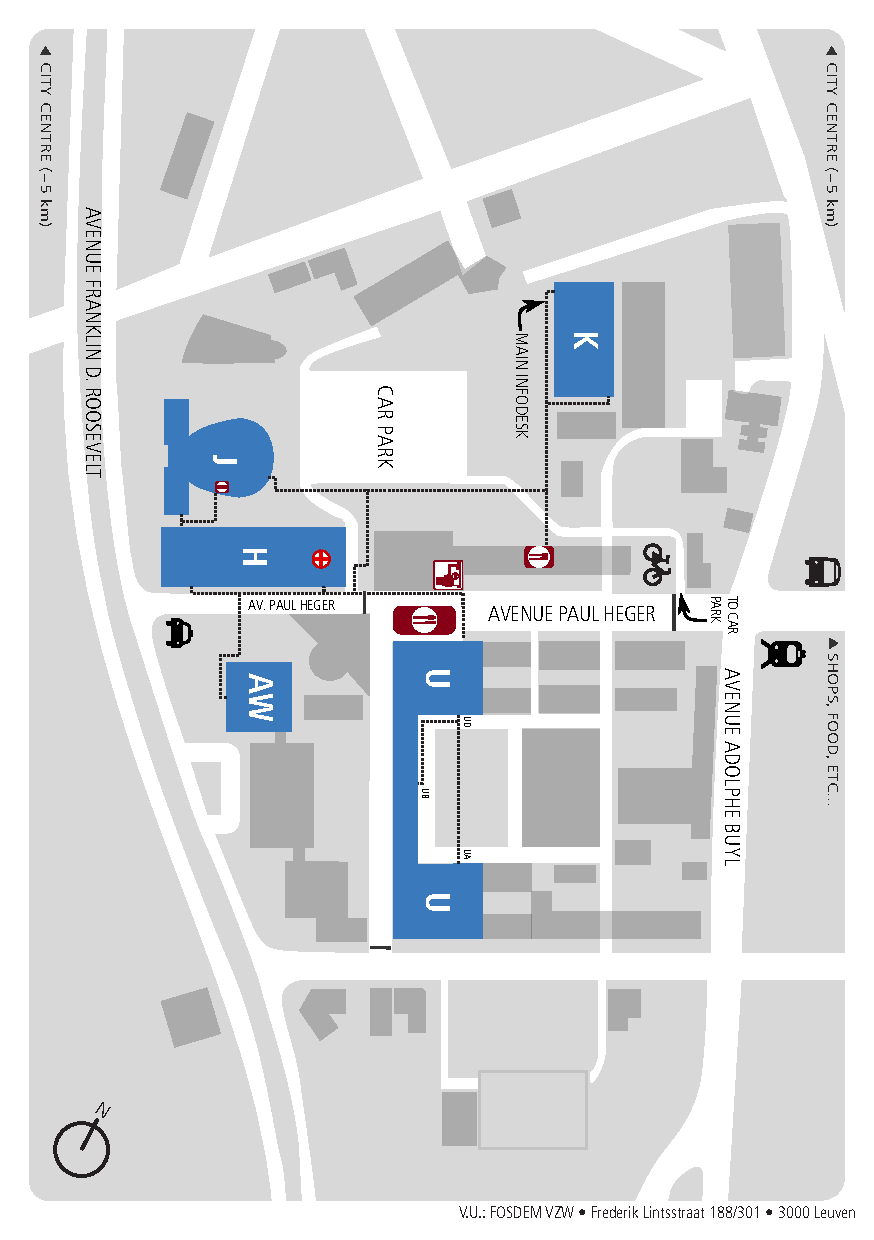
\includegraphics[width=\textwidth]{artwork/campusmap}

\end{document}
